\documentclass{article}

% Camera-ready, GenAI4Health 2026 (NeurIPS workshop, non-archival). The workshop's package loads
% neurips_2026 with [dblblindworkshop,final] and sets the workshop title and first-page notice.
\usepackage{genai4health_2026}

\usepackage[utf8]{inputenc}
\usepackage[T1]{fontenc}
\usepackage{amsmath,amssymb}
\usepackage{graphicx}
\usepackage{booktabs}
\usepackage{microtype}
\usepackage{xcolor}
\usepackage[colorlinks=true,allcolors=blue]{hyperref}
\graphicspath{{figures/}}

% Every result number comes from \val{key} or a table under tables/, both written by
% paper/make_numbers.py from the result files; none is typed here. An unknown key prints red.
% \todo marks text still to write; preflight fails on either.
\newcommand{\todo}[1]{\textcolor{red}{[#1]}}
\makeatletter
\newcommand{\defval}[2]{\expandafter\def\csname val@#1\endcsname{#2}}
\newcommand{\val}[1]{\ifcsname val@#1\endcsname\csname val@#1\endcsname\else
  \textcolor{red}{??\detokenize{#1}}\PackageWarning{numbers}{undefined value #1}\fi}
\makeatother
% generated by paper/make_numbers.py; do not edit
\defval{a1.img}{\ensuremath{1.19}}
\defval{a1.txt}{\ensuremath{0.10}}
\defval{alt.last.changed}{186}
\defval{alt.norm.max}{\ensuremath{0.28}}
\defval{alt.norm.min}{\ensuremath{0.19}}
\defval{alt.nsamples}{8{,}000}
\defval{attn.apfp.best}{\ensuremath{0.557}}
\defval{attn.apfp.n}{20}
\defval{attn.apfp.nrem}{12}
\defval{attn.apfp.rho}{\ensuremath{-0.076}}
\defval{attn.apfp.shuf}{\ensuremath{+0.002}}
\defval{attn.eff.bestmax}{\ensuremath{0.998}}
\defval{attn.fp.best}{\ensuremath{0.416}}
\defval{attn.fp.n}{20}
\defval{attn.fp.nrem}{10}
\defval{attn.fp.rho}{\ensuremath{-0.101}}
\defval{attn.fp.shuf}{\ensuremath{-0.010}}
\defval{attn.perpatch}{\ensuremath{-0.067}}
\defval{attn.perpatch.ci}{\ensuremath{-0.067\;[-0.158,\,+0.029]}}
\defval{attn.perpatch.n}{20}
\defval{attn.perpatch.shuf}{\ensuremath{-0.009}}
\defval{attn.ptx.bestmax}{\ensuremath{0.996}}
\defval{attn.rhomax}{\ensuremath{+0.009}}
\defval{attn.rhomin}{\ensuremath{-0.109}}
\defval{attn.shufmax}{\ensuremath{+0.002}}
\defval{attn.shufmin}{\ensuremath{-0.030}}
\defval{attn.tpcard.best}{\ensuremath{0.244}}
\defval{attn.tpcard.n}{20}
\defval{attn.tpcard.nrem}{5}
\defval{attn.tpcard.rho}{\ensuremath{-0.087}}
\defval{attn.tpcard.shuf}{\ensuremath{+0.002}}
\defval{attn.tpeff.best}{\ensuremath{0.147}}
\defval{attn.tpeff.n}{20}
\defval{attn.tpeff.nrem}{5}
\defval{attn.tpeff.rho}{\ensuremath{+0.009}}
\defval{attn.tpeff.shuf}{\ensuremath{-0.005}}
\defval{attn.tpptx.best}{\ensuremath{0.282}}
\defval{attn.tpptx.n}{20}
\defval{attn.tpptx.nrem}{6}
\defval{attn.tpptx.rho}{\ensuremath{-0.109}}
\defval{attn.tpptx.shuf}{\ensuremath{-0.030}}
\defval{ceil.highmax}{\ensuremath{0.09}}
\defval{ceil.highmin}{\ensuremath{0.03}}
\defval{ceil.lowmax}{\ensuremath{0.38}}
\defval{ceil.lowmin}{\ensuremath{0.29}}
\defval{ceil.rhomax}{\ensuremath{0.90}}
\defval{ceil.rhomin}{\ensuremath{0.87}}
\defval{ceil.sdroptinymax}{\ensuremath{0.21}}
\defval{ceil.sdroptinymin}{\ensuremath{0.16}}
\defval{ceil.tinymax}{34}
\defval{ceil.tinymin}{30}
\defval{clamp.nlast.max}{25}
\defval{clamp.nlast.mean}{\ensuremath{21}}
\defval{clamp.nlast.min}{19}
\defval{clt.params}{6.24}
\defval{clt.span0.params}{0.36}
\defval{clt.unused}{2.94}
\defval{clt.used}{3.30}
\defval{compute.e2}{8}
\defval{compute.e4}{47}
\defval{compute.e5}{48}
\defval{compute.e6cx}{21}
\defval{compute.e6mg}{33}
\defval{compute.e7cx}{59}
\defval{compute.e7mg}{69}
\defval{e2.ablate.banked}{\ensuremath{0.077}}
\defval{e2.ablate.greedyno}{4}
\defval{e2.ablate.s}{\ensuremath{0.84}}
\defval{e2.ablate.v}{\textsc{disagrees}}
\defval{e2.base.banked}{\ensuremath{0.032}}
\defval{e2.base.greedyno}{0}
\defval{e2.base.s}{\ensuremath{0.98}}
\defval{e2.black.banked}{\ensuremath{0.034}}
\defval{e2.black.greedyno}{11}
\defval{e2.black.s}{\ensuremath{0.33}}
\defval{e2.blur.banked}{\ensuremath{0.088}}
\defval{e2.blur.greedyno}{2}
\defval{e2.blur.s}{\ensuremath{0.90}}
\defval{e2.border.banked}{\ensuremath{0.054}}
\defval{e2.border.greedyno}{0}
\defval{e2.border.s}{\ensuremath{0.97}}
\defval{e2.greedy.total}{160}
\defval{e2.mean.banked}{\ensuremath{0.094}}
\defval{e2.mean.greedyno}{10}
\defval{e2.mean.s}{\ensuremath{0.44}}
\defval{e2.n}{20}
\defval{e2.nsamples}{10}
\defval{e2.scale1.banked}{\ensuremath{0.108}}
\defval{e2.scale1.greedyno}{4}
\defval{e2.scale1.s}{\ensuremath{0.73}}
\defval{e2.scale1.v}{\textsc{disagrees}}
\defval{e2.scale2.banked}{\ensuremath{0.107}}
\defval{e2.scale2.greedyno}{3}
\defval{e2.scale2.s}{\ensuremath{0.69}}
\defval{e2.scale2.v}{\textsc{disagrees}}
\defval{e2.torch}{2.14.1}
\defval{e2.transformers}{5.14.1}
\defval{e3.amp.cardminuseff}{\ensuremath{0.010}}
\defval{e3.amp.p.eff}{\ensuremath{0.039}}
\defval{e3.amp.p.ptx}{\ensuremath{0.56}}
\defval{e3.amp.verdict}{\textsc{no effect}}
\defval{e3.amp.vsrandom.norm}{\ensuremath{0.045}}
\defval{e3.amp.vsrandom.raw}{\ensuremath{0.093}}
\defval{e3.jac.activation.20}{\ensuremath{0.770}}
\defval{e3.jac.activation.320}{\ensuremath{0.939}}
\defval{e3.jac.activation.80}{\ensuremath{0.944}}
\defval{e3.jac.contrast.20}{\ensuremath{0.194}}
\defval{e3.jac.contrast.320}{\ensuremath{0.331}}
\defval{e3.jac.contrast.80}{\ensuremath{0.284}}
\defval{e3.ndonor}{8}
\defval{e3.nfilms}{12}
\defval{e3.old.card}{\ensuremath{0.126}}
\defval{e3.old.eff}{\ensuremath{0.124}}
\defval{e3.old.ptx}{\ensuremath{0.194}}
\defval{e3.overlap.max}{79}
\defval{e3.overlap.min}{77}
\defval{e3.verdict}{\textsc{still finding-agnostic}}
\defval{e4.maxtok}{128}
\defval{e4.nsamples}{50}
\defval{e5.S1}{\textsc{contrastive sets inert}}
\defval{e5.S1.a}{\ensuremath{+0.00\;[-0.01,\,+0.01]}}
\defval{e5.S1.b}{\ensuremath{-0.01\;[-0.04,\,+0.02]}}
\defval{e5.S1.cardrand}{\ensuremath{+0.01\;[+0.00,\,+0.02]}}
\defval{e5.S1.effrand}{\ensuremath{-0.01\;[-0.04,\,+0.02]}}
\defval{e5.S2}{\textsc{contrast inert on fp}}
\defval{e5.S2.ci}{\ensuremath{+0.03\;[-0.02,\,+0.07]}}
\defval{e5.S3}{\textsc{unresolved}}
\defval{e5.S3.ci}{\ensuremath{+0.08\;[+0.01,\,+0.16]}}
\defval{e5.S3.tpcard}{\textsc{unresolved}}
\defval{e5.S3.tpcard.ci}{\ensuremath{+0.06\;[-0.01,\,+0.17]}}
\defval{e5.S3.tpeff}{\textsc{location matters}}
\defval{e5.S3.tpeff.ci}{\ensuremath{+0.27\;[+0.11,\,+0.43]}}
\defval{e5.fp.base.raw}{\ensuremath{0.82}}
\defval{e5.fp.base.s}{\ensuremath{0.95}}
\defval{e5.fp.border.nactive}{\ensuremath{80.0}}
\defval{e5.fp.border.normv}{\textsc{misreads}}
\defval{e5.fp.border.overlap}{\ensuremath{68.5}}
\defval{e5.fp.border.raw}{\ensuremath{0.62}}
\defval{e5.fp.border.rawv}{\textsc{unresolved}}
\defval{e5.fp.border.sdrop}{\ensuremath{0.19\;[0.13,\,0.26]}}
\defval{e5.fp.concard.nactive}{\ensuremath{80.0}}
\defval{e5.fp.concard.normv}{\textsc{misreads}}
\defval{e5.fp.concard.overlap}{\ensuremath{24.9}}
\defval{e5.fp.concard.raw}{\ensuremath{0.81}}
\defval{e5.fp.concard.rawv}{\textsc{misreads}}
\defval{e5.fp.concard.sdrop}{\ensuremath{0.07\;[0.03,\,0.11]}}
\defval{e5.fp.coneff.nactive}{\ensuremath{79.6}}
\defval{e5.fp.coneff.normv}{\textsc{unresolved}}
\defval{e5.fp.coneff.overlap}{\ensuremath{25.0}}
\defval{e5.fp.coneff.raw}{\ensuremath{0.88}}
\defval{e5.fp.coneff.rawv}{\textsc{misreads}}
\defval{e5.fp.coneff.sdrop}{\ensuremath{0.04\;[0.02,\,0.06]}}
\defval{e5.fp.evid.nactive}{\ensuremath{80.0}}
\defval{e5.fp.evid.normv}{\textsc{misreads}}
\defval{e5.fp.evid.overlap}{\ensuremath{68.0}}
\defval{e5.fp.evid.raw}{\ensuremath{0.55}}
\defval{e5.fp.evid.rawv}{\textsc{unresolved}}
\defval{e5.fp.evid.sdrop}{\ensuremath{0.27\;[0.19,\,0.36]}}
\defval{e5.fp.n}{40}
\defval{e5.fp.rand.nactive}{\ensuremath{80.0}}
\defval{e5.fp.rand.normv}{\textsc{unresolved}}
\defval{e5.fp.rand.overlap}{\ensuremath{4.4}}
\defval{e5.fp.rand.raw}{\ensuremath{0.78}}
\defval{e5.fp.rand.rawv}{\textsc{tracks}}
\defval{e5.fp.rand.sdrop}{\ensuremath{0.04\;[0.01,\,0.07]}}
\defval{e5.fp.top.nactive}{\ensuremath{80.0}}
\defval{e5.fp.top.normv}{\textsc{misreads}}
\defval{e5.fp.top.overlap}{\ensuremath{80.0}}
\defval{e5.fp.top.raw}{\ensuremath{0.56}}
\defval{e5.fp.top.rawv}{\textsc{unresolved}}
\defval{e5.fp.top.sdrop}{\ensuremath{0.23\;[0.16,\,0.30]}}
\defval{e5.jaccon}{\ensuremath{0.231}}
\defval{e5.ndonor}{16}
\defval{e5.nsamples}{30}
\defval{e5.tpcard.base.raw}{\ensuremath{0.97}}
\defval{e5.tpcard.base.s}{\ensuremath{0.99}}
\defval{e5.tpcard.border.nactive}{\ensuremath{80.0}}
\defval{e5.tpcard.border.normv}{\textsc{tracks}}
\defval{e5.tpcard.border.overlap}{\ensuremath{70.3}}
\defval{e5.tpcard.border.raw}{\ensuremath{0.92}}
\defval{e5.tpcard.border.rawv}{\textsc{unresolved}}
\defval{e5.tpcard.border.sdrop}{\ensuremath{0.02\;[0.01,\,0.04]}}
\defval{e5.tpcard.concard.nactive}{\ensuremath{79.7}}
\defval{e5.tpcard.concard.normv}{\textsc{tracks}}
\defval{e5.tpcard.concard.overlap}{\ensuremath{24.2}}
\defval{e5.tpcard.concard.raw}{\ensuremath{0.97}}
\defval{e5.tpcard.concard.rawv}{\textsc{tracks}}
\defval{e5.tpcard.concard.sdrop}{\ensuremath{0.00\;[0.00,\,0.01]}}
\defval{e5.tpcard.coneff.nactive}{\ensuremath{78.7}}
\defval{e5.tpcard.coneff.normv}{\textsc{tracks}}
\defval{e5.tpcard.coneff.overlap}{\ensuremath{23.6}}
\defval{e5.tpcard.coneff.raw}{\ensuremath{0.99}}
\defval{e5.tpcard.coneff.rawv}{\textsc{tracks}}
\defval{e5.tpcard.coneff.sdrop}{\ensuremath{0.00\;[-0.01,\,0.01]}}
\defval{e5.tpcard.evid.nactive}{\ensuremath{80.0}}
\defval{e5.tpcard.evid.normv}{\textsc{misreads}}
\defval{e5.tpcard.evid.overlap}{\ensuremath{65.3}}
\defval{e5.tpcard.evid.raw}{\ensuremath{0.84}}
\defval{e5.tpcard.evid.rawv}{\textsc{unresolved}}
\defval{e5.tpcard.evid.sdrop}{\ensuremath{0.09\;[0.02,\,0.19]}}
\defval{e5.tpcard.n}{20}
\defval{e5.tpcard.rand.nactive}{\ensuremath{80.0}}
\defval{e5.tpcard.rand.normv}{\textsc{tracks}}
\defval{e5.tpcard.rand.overlap}{\ensuremath{4.5}}
\defval{e5.tpcard.rand.raw}{\ensuremath{0.96}}
\defval{e5.tpcard.rand.rawv}{\textsc{tracks}}
\defval{e5.tpcard.rand.sdrop}{\ensuremath{-0.00\;[-0.01,\,0.00]}}
\defval{e5.tpcard.top.nactive}{\ensuremath{80.0}}
\defval{e5.tpcard.top.normv}{\textsc{unresolved}}
\defval{e5.tpcard.top.overlap}{\ensuremath{80.0}}
\defval{e5.tpcard.top.raw}{\ensuremath{0.89}}
\defval{e5.tpcard.top.rawv}{\textsc{unresolved}}
\defval{e5.tpcard.top.sdrop}{\ensuremath{0.04\;[0.02,\,0.07]}}
\defval{e5.tpeff.base.raw}{\ensuremath{0.92}}
\defval{e5.tpeff.base.s}{\ensuremath{0.95}}
\defval{e5.tpeff.border.nactive}{\ensuremath{80.0}}
\defval{e5.tpeff.border.normv}{\textsc{misreads}}
\defval{e5.tpeff.border.overlap}{\ensuremath{67.2}}
\defval{e5.tpeff.border.raw}{\ensuremath{0.79}}
\defval{e5.tpeff.border.rawv}{\textsc{unresolved}}
\defval{e5.tpeff.border.sdrop}{\ensuremath{0.10\;[0.04,\,0.19]}}
\defval{e5.tpeff.concard.nactive}{\ensuremath{79.6}}
\defval{e5.tpeff.concard.normv}{\textsc{unresolved}}
\defval{e5.tpeff.concard.overlap}{\ensuremath{24.4}}
\defval{e5.tpeff.concard.raw}{\ensuremath{0.87}}
\defval{e5.tpeff.concard.rawv}{\textsc{tracks}}
\defval{e5.tpeff.concard.sdrop}{\ensuremath{0.03\;[0.01,\,0.06]}}
\defval{e5.tpeff.coneff.nactive}{\ensuremath{79.1}}
\defval{e5.tpeff.coneff.normv}{\textsc{unresolved}}
\defval{e5.tpeff.coneff.overlap}{\ensuremath{26.3}}
\defval{e5.tpeff.coneff.raw}{\ensuremath{0.91}}
\defval{e5.tpeff.coneff.rawv}{\textsc{unresolved}}
\defval{e5.tpeff.coneff.sdrop}{\ensuremath{0.02\;[-0.01,\,0.06]}}
\defval{e5.tpeff.evid.nactive}{\ensuremath{80.0}}
\defval{e5.tpeff.evid.normv}{\textsc{misreads}}
\defval{e5.tpeff.evid.overlap}{\ensuremath{65.3}}
\defval{e5.tpeff.evid.raw}{\ensuremath{0.55}}
\defval{e5.tpeff.evid.rawv}{\textsc{unresolved}}
\defval{e5.tpeff.evid.sdrop}{\ensuremath{0.37\;[0.21,\,0.53]}}
\defval{e5.tpeff.n}{20}
\defval{e5.tpeff.rand.nactive}{\ensuremath{80.0}}
\defval{e5.tpeff.rand.normv}{\textsc{unresolved}}
\defval{e5.tpeff.rand.overlap}{\ensuremath{5.0}}
\defval{e5.tpeff.rand.raw}{\ensuremath{0.89}}
\defval{e5.tpeff.rand.rawv}{\textsc{tracks}}
\defval{e5.tpeff.rand.sdrop}{\ensuremath{0.03\;[-0.00,\,0.08]}}
\defval{e5.tpeff.top.nactive}{\ensuremath{80.0}}
\defval{e5.tpeff.top.normv}{\textsc{misreads}}
\defval{e5.tpeff.top.overlap}{\ensuremath{80.0}}
\defval{e5.tpeff.top.raw}{\ensuremath{0.73}}
\defval{e5.tpeff.top.rawv}{\textsc{unresolved}}
\defval{e5.tpeff.top.sdrop}{\ensuremath{0.17\;[0.06,\,0.30]}}
\defval{e6.cx.card.acc.greedy}{\ensuremath{0.87}}
\defval{e6.cx.card.acc.norm}{\ensuremath{0.86}}
\defval{e6.cx.card.acc.raw}{\ensuremath{0.87}}
\defval{e6.cx.card.acc.s}{\ensuremath{0.86}}
\defval{e6.cx.card.auc.greedy}{\ensuremath{0.866\;[0.813,\,0.912]}}
\defval{e6.cx.card.auc.norm}{\ensuremath{0.955\;[0.928,\,0.977]}}
\defval{e6.cx.card.auc.raw}{\ensuremath{0.955\;[0.928,\,0.977]}}
\defval{e6.cx.card.auc.s}{\ensuremath{0.954\;[0.926,\,0.977]}}
\defval{e6.cx.card.dis.norm}{2}
\defval{e6.cx.card.dis.raw}{1}
\defval{e6.cx.card.greedynone}{0}
\defval{e6.cx.card.mass}{\ensuremath{1.00}}
\defval{e6.cx.card.matched.norm}{\ensuremath{-0.007\;[-0.021,\,+0.005]}}
\defval{e6.cx.card.matched.raw}{\ensuremath{-0.007\;[-0.022,\,+0.006]}}
\defval{e6.cx.card.nneg}{93}
\defval{e6.cx.card.normvs}{\ensuremath{+0.001\;[-0.008,\,+0.008]}}
\defval{e6.cx.card.npos}{93}
\defval{e6.cx.card.rawvs}{\ensuremath{+0.001\;[-0.008,\,+0.009]}}
\defval{e6.cx.card.s0n}{52}
\defval{e6.cx.card.s0pos}{0}
\defval{e6.cx.eff.acc.greedy}{\ensuremath{0.83}}
\defval{e6.cx.eff.acc.norm}{\ensuremath{0.82}}
\defval{e6.cx.eff.acc.raw}{\ensuremath{0.83}}
\defval{e6.cx.eff.acc.s}{\ensuremath{0.81}}
\defval{e6.cx.eff.auc.greedy}{\ensuremath{0.830\;[0.777,\,0.880]}}
\defval{e6.cx.eff.auc.norm}{\ensuremath{0.880\;[0.831,\,0.923]}}
\defval{e6.cx.eff.auc.raw}{\ensuremath{0.880\;[0.831,\,0.923]}}
\defval{e6.cx.eff.auc.s}{\ensuremath{0.865\;[0.814,\,0.911]}}
\defval{e6.cx.eff.dis.norm}{8}
\defval{e6.cx.eff.dis.raw}{9}
\defval{e6.cx.eff.greedynone}{0}
\defval{e6.cx.eff.mass}{\ensuremath{1.00}}
\defval{e6.cx.eff.matched.norm}{\ensuremath{+0.004\;[-0.017,\,+0.025]}}
\defval{e6.cx.eff.matched.raw}{\ensuremath{+0.004\;[-0.018,\,+0.025]}}
\defval{e6.cx.eff.nneg}{100}
\defval{e6.cx.eff.normvs}{\ensuremath{+0.016\;[+0.002,\,+0.030]}}
\defval{e6.cx.eff.npos}{100}
\defval{e6.cx.eff.rawvs}{\ensuremath{+0.016\;[+0.003,\,+0.030]}}
\defval{e6.cx.eff.s0auc}{\ensuremath{0.77}}
\defval{e6.cx.eff.s0n}{14}
\defval{e6.cx.eff.s0pos}{1}
\defval{e6.cx.massmax}{\ensuremath{1.00}}
\defval{e6.cx.massmin}{\ensuremath{1.00}}
\defval{e6.cx.nlevels}{21}
\defval{e6.cx.nonesamples}{14}
\defval{e6.cx.nsamples}{20}
\defval{e6.cx.nsamplestotal}{10{,}000}
\defval{e6.cx.ptx.acc.greedy}{\ensuremath{0.73}}
\defval{e6.cx.ptx.acc.norm}{\ensuremath{0.73}}
\defval{e6.cx.ptx.acc.raw}{\ensuremath{0.73}}
\defval{e6.cx.ptx.acc.s}{\ensuremath{0.75}}
\defval{e6.cx.ptx.auc.greedy}{\ensuremath{0.728\;[0.652,\,0.800]}}
\defval{e6.cx.ptx.auc.norm}{\ensuremath{0.864\;[0.795,\,0.929]}}
\defval{e6.cx.ptx.auc.raw}{\ensuremath{0.863\;[0.793,\,0.928]}}
\defval{e6.cx.ptx.auc.s}{\ensuremath{0.834\;[0.757,\,0.908]}}
\defval{e6.cx.ptx.dis.norm}{2}
\defval{e6.cx.ptx.dis.raw}{2}
\defval{e6.cx.ptx.greedynone}{0}
\defval{e6.cx.ptx.mass}{\ensuremath{1.00}}
\defval{e6.cx.ptx.matched.norm}{\ensuremath{+0.013\;[-0.024,\,+0.051]}}
\defval{e6.cx.ptx.matched.raw}{\ensuremath{+0.013\;[-0.026,\,+0.052]}}
\defval{e6.cx.ptx.nneg}{57}
\defval{e6.cx.ptx.normvs}{\ensuremath{+0.030\;[+0.005,\,+0.058]}}
\defval{e6.cx.ptx.npos}{57}
\defval{e6.cx.ptx.rawvs}{\ensuremath{+0.028\;[+0.003,\,+0.056]}}
\defval{e6.cx.ptx.s0auc}{\ensuremath{0.49}}
\defval{e6.cx.ptx.s0n}{21}
\defval{e6.cx.ptx.s0pos}{5}
\defval{e6.cx.tiedmax}{47\%}
\defval{e6.cx.tiedmin}{20\%}
\defval{e6.cx.verdict}{\textsc{unresolved}}
\defval{e6.cxnl.n}{25}
\defval{e6.cxnl.no}{3}
\defval{e6.cxnl.yes}{22}
\defval{e6.mg.card.acc.greedy}{\ensuremath{0.76}}
\defval{e6.mg.card.acc.norm}{\ensuremath{0.84}}
\defval{e6.mg.card.acc.raw}{\ensuremath{0.86}}
\defval{e6.mg.card.acc.s}{\ensuremath{0.85}}
\defval{e6.mg.card.auc.greedy}{\ensuremath{0.832\;[0.774,\,0.885]}}
\defval{e6.mg.card.auc.norm}{\ensuremath{0.925\;[0.883,\,0.959]}}
\defval{e6.mg.card.auc.raw}{\ensuremath{0.921\;[0.877,\,0.957]}}
\defval{e6.mg.card.auc.s}{\ensuremath{0.883\;[0.831,\,0.931]}}
\defval{e6.mg.card.dis.norm}{3}
\defval{e6.mg.card.dis.raw}{8}
\defval{e6.mg.card.greedynone}{16}
\defval{e6.mg.card.mass}{\ensuremath{0.61}}
\defval{e6.mg.card.matched.norm}{\ensuremath{-0.018\;[-0.045,\,+0.009]}}
\defval{e6.mg.card.matched.raw}{\ensuremath{+0.003\;[-0.017,\,+0.023]}}
\defval{e6.mg.card.nneg}{93}
\defval{e6.mg.card.normvs}{\ensuremath{+0.042\;[+0.016,\,+0.069]}}
\defval{e6.mg.card.npos}{93}
\defval{e6.mg.card.rawvs}{\ensuremath{+0.038\;[+0.010,\,+0.067]}}
\defval{e6.mg.card.s0auc}{\ensuremath{0.88}}
\defval{e6.mg.card.s0n}{69}
\defval{e6.mg.card.s0pos}{10}
\defval{e6.mg.eff.acc.greedy}{\ensuremath{0.80}}
\defval{e6.mg.eff.acc.norm}{\ensuremath{0.78}}
\defval{e6.mg.eff.acc.raw}{\ensuremath{0.76}}
\defval{e6.mg.eff.acc.s}{\ensuremath{0.78}}
\defval{e6.mg.eff.auc.greedy}{\ensuremath{0.799\;[0.744,\,0.853]}}
\defval{e6.mg.eff.auc.norm}{\ensuremath{0.851\;[0.794,\,0.903]}}
\defval{e6.mg.eff.auc.raw}{\ensuremath{0.857\;[0.801,\,0.908]}}
\defval{e6.mg.eff.auc.s}{\ensuremath{0.809\;[0.750,\,0.866]}}
\defval{e6.mg.eff.dis.norm}{1}
\defval{e6.mg.eff.dis.raw}{7}
\defval{e6.mg.eff.greedynone}{1}
\defval{e6.mg.eff.mass}{\ensuremath{0.55}}
\defval{e6.mg.eff.matched.norm}{\ensuremath{-0.008\;[-0.030,\,+0.014]}}
\defval{e6.mg.eff.matched.raw}{\ensuremath{-0.013\;[-0.042,\,+0.014]}}
\defval{e6.mg.eff.nneg}{100}
\defval{e6.mg.eff.normvs}{\ensuremath{+0.042\;[+0.013,\,+0.071]}}
\defval{e6.mg.eff.npos}{100}
\defval{e6.mg.eff.rawvs}{\ensuremath{+0.048\;[+0.021,\,+0.077]}}
\defval{e6.mg.eff.s0auc}{\ensuremath{0.79}}
\defval{e6.mg.eff.s0n}{88}
\defval{e6.mg.eff.s0pos}{18}
\defval{e6.mg.massmax}{\ensuremath{0.65}}
\defval{e6.mg.massmin}{\ensuremath{0.55}}
\defval{e6.mg.nlevels}{21}
\defval{e6.mg.nonesamples}{492}
\defval{e6.mg.nsamples}{20}
\defval{e6.mg.nsamplestotal}{10{,}000}
\defval{e6.mg.ptx.acc.greedy}{\ensuremath{0.64}}
\defval{e6.mg.ptx.acc.norm}{\ensuremath{0.64}}
\defval{e6.mg.ptx.acc.raw}{\ensuremath{0.63}}
\defval{e6.mg.ptx.acc.s}{\ensuremath{0.64}}
\defval{e6.mg.ptx.auc.greedy}{\ensuremath{0.643\;[0.573,\,0.714]}}
\defval{e6.mg.ptx.auc.norm}{\ensuremath{0.625\;[0.512,\,0.732]}}
\defval{e6.mg.ptx.auc.raw}{\ensuremath{0.622\;[0.507,\,0.730]}}
\defval{e6.mg.ptx.auc.s}{\ensuremath{0.685\;[0.603,\,0.765]}}
\defval{e6.mg.ptx.dis.norm}{0}
\defval{e6.mg.ptx.dis.raw}{1}
\defval{e6.mg.ptx.greedynone}{1}
\defval{e6.mg.ptx.mass}{\ensuremath{0.65}}
\defval{e6.mg.ptx.matched.norm}{\ensuremath{-0.028\;[-0.071,\,+0.012]}}
\defval{e6.mg.ptx.matched.raw}{\ensuremath{-0.029\;[-0.074,\,+0.012]}}
\defval{e6.mg.ptx.nneg}{57}
\defval{e6.mg.ptx.normvs}{\ensuremath{-0.060\;[-0.121,\,+0.002]}}
\defval{e6.mg.ptx.npos}{57}
\defval{e6.mg.ptx.rawvs}{\ensuremath{-0.064\;[-0.126,\,-0.002]}}
\defval{e6.mg.ptx.s0auc}{\ensuremath{0.34}}
\defval{e6.mg.ptx.s0n}{77}
\defval{e6.mg.ptx.s0pos}{29}
\defval{e6.mg.tiedmax}{82\%}
\defval{e6.mg.tiedmin}{76\%}
\defval{e6.mg.verdict}{\textsc{readout changes the evaluation}}
\defval{e6.npairs}{500}
\defval{e6.rank.card.greedy}{\ensuremath{-0.034\;[-0.092,\,+0.022]}}
\defval{e6.rank.card.norm}{\ensuremath{-0.030\;[-0.060,\,-0.002]}}
\defval{e6.rank.card.raw}{\ensuremath{-0.034\;[-0.067,\,-0.004]}}
\defval{e6.rank.card.s}{\ensuremath{-0.071\;[-0.115,\,-0.031]}}
\defval{e6.rank.eff.greedy}{\ensuremath{-0.031\;[-0.072,\,+0.010]}}
\defval{e6.rank.eff.norm}{\ensuremath{-0.029\;[-0.062,\,+0.001]}}
\defval{e6.rank.eff.raw}{\ensuremath{-0.024\;[-0.055,\,+0.006]}}
\defval{e6.rank.eff.s}{\ensuremath{-0.056\;[-0.098,\,-0.019]}}
\defval{e6.rank.model}{CheXagent-2 3B}
\defval{e6.rank.ptx.greedy}{\ensuremath{-0.085\;[-0.144,\,-0.027]}}
\defval{e6.rank.ptx.norm}{\ensuremath{-0.239\;[-0.336,\,-0.147]}}
\defval{e6.rank.ptx.raw}{\ensuremath{-0.241\;[-0.338,\,-0.150]}}
\defval{e6.rank.ptx.s}{\ensuremath{-0.149\;[-0.223,\,-0.072]}}
\defval{e6.rank.verdict}{\textsc{ranking differs in significance}}
\defval{e6.res.maxabs}{\ensuremath{0.03}}
\defval{e6.res.rank.card}{\ensuremath{-0.061\;[-0.105,\,-0.020]}}
\defval{e6.res.rank.eff}{\ensuremath{-0.073\;[-0.112,\,-0.032]}}
\defval{e6.res.rank.ptx}{\ensuremath{-0.191\;[-0.260,\,-0.120]}}
\defval{e7.cx.card.D.norm}{\ensuremath{-0.001\;[-0.009,\,+0.006]}}
\defval{e7.cx.card.D.raw}{\ensuremath{-0.001\;[-0.009,\,+0.006]}}
\defval{e7.cx.card.auc.norm}{\ensuremath{0.904}}
\defval{e7.cx.card.auc.raw}{\ensuremath{0.903}}
\defval{e7.cx.card.auc.s}{\ensuremath{0.904}}
\defval{e7.cx.card.eauc.norm}{\ensuremath{0.905}}
\defval{e7.cx.card.eauc.raw}{\ensuremath{0.905}}
\defval{e7.cx.card.nneg}{100}
\defval{e7.cx.card.npos}{100}
\defval{e7.cx.card.s0auc}{\ensuremath{0.39}}
\defval{e7.cx.card.s0n}{46}
\defval{e7.cx.card.s0pos}{4}
\defval{e7.cx.card.unmatched.norm}{\ensuremath{-0.000\;[-0.010,\,+0.009]}}
\defval{e7.cx.card.unmatched.raw}{\ensuremath{+0.000\;[-0.010,\,+0.009]}}
\defval{e7.cx.e6rule}{\textsc{unresolved}}
\defval{e7.cx.eff.D.norm}{\ensuremath{-0.000\;[-0.010,\,+0.010]}}
\defval{e7.cx.eff.D.raw}{\ensuremath{-0.000\;[-0.010,\,+0.010]}}
\defval{e7.cx.eff.auc.norm}{\ensuremath{0.850}}
\defval{e7.cx.eff.auc.raw}{\ensuremath{0.850}}
\defval{e7.cx.eff.auc.s}{\ensuremath{0.847}}
\defval{e7.cx.eff.eauc.norm}{\ensuremath{0.848}}
\defval{e7.cx.eff.eauc.raw}{\ensuremath{0.848}}
\defval{e7.cx.eff.nneg}{100}
\defval{e7.cx.eff.npos}{100}
\defval{e7.cx.eff.s0n}{2}
\defval{e7.cx.eff.s0pos}{0}
\defval{e7.cx.eff.unmatched.norm}{\ensuremath{-0.003\;[-0.012,\,+0.007]}}
\defval{e7.cx.eff.unmatched.raw}{\ensuremath{-0.002\;[-0.011,\,+0.008]}}
\defval{e7.cx.gapmax}{\ensuremath{0.018}}
\defval{e7.cx.gapmin}{\ensuremath{-0.000}}
\defval{e7.cx.gatemax}{\ensuremath{0.000}}
\defval{e7.cx.massmax}{\ensuremath{1.00}}
\defval{e7.cx.massmin}{\ensuremath{1.00}}
\defval{e7.cx.maxbound}{\ensuremath{0.03}}
\defval{e7.cx.maxhw}{\ensuremath{0.022}}
\defval{e7.cx.nonesamples}{35}
\defval{e7.cx.nsamplestotal}{30{,}000}
\defval{e7.cx.outbinmax}{4\%}
\defval{e7.cx.outbinmin}{2\%}
\defval{e7.cx.ptx.D.norm}{\ensuremath{-0.005\;[-0.028,\,+0.016]}}
\defval{e7.cx.ptx.D.raw}{\ensuremath{-0.005\;[-0.028,\,+0.016]}}
\defval{e7.cx.ptx.auc.norm}{\ensuremath{0.862}}
\defval{e7.cx.ptx.auc.raw}{\ensuremath{0.862}}
\defval{e7.cx.ptx.auc.s}{\ensuremath{0.845}}
\defval{e7.cx.ptx.eauc.norm}{\ensuremath{0.850}}
\defval{e7.cx.ptx.eauc.raw}{\ensuremath{0.850}}
\defval{e7.cx.ptx.nneg}{100}
\defval{e7.cx.ptx.npos}{100}
\defval{e7.cx.ptx.s0n}{7}
\defval{e7.cx.ptx.s0pos}{0}
\defval{e7.cx.ptx.unmatched.norm}{\ensuremath{-0.018\;[-0.043,\,+0.006]}}
\defval{e7.cx.ptx.unmatched.raw}{\ensuremath{-0.018\;[-0.042,\,+0.007]}}
\defval{e7.cx.tiedmax}{36\%}
\defval{e7.cx.tiedmin}{5\%}
\defval{e7.cx.verdict}{\textsc{answers follow the readout}}
\defval{e7.maxabsD}{\ensuremath{0.023}}
\defval{e7.maxhw}{\ensuremath{0.046}}
\defval{e7.mg.card.D.norm}{\ensuremath{-0.007\;[-0.031,\,+0.016]}}
\defval{e7.mg.card.D.raw}{\ensuremath{+0.003\;[-0.017,\,+0.025]}}
\defval{e7.mg.card.auc.norm}{\ensuremath{0.885}}
\defval{e7.mg.card.auc.raw}{\ensuremath{0.886}}
\defval{e7.mg.card.auc.s}{\ensuremath{0.854}}
\defval{e7.mg.card.eauc.norm}{\ensuremath{0.862}}
\defval{e7.mg.card.eauc.raw}{\ensuremath{0.851}}
\defval{e7.mg.card.nneg}{100}
\defval{e7.mg.card.npos}{100}
\defval{e7.mg.card.s0auc}{\ensuremath{0.73}}
\defval{e7.mg.card.s0n}{64}
\defval{e7.mg.card.s0pos}{10}
\defval{e7.mg.card.unmatched.norm}{\ensuremath{-0.031\;[-0.062,\,-0.003]}}
\defval{e7.mg.card.unmatched.raw}{\ensuremath{-0.032\;[-0.061,\,-0.006]}}
\defval{e7.mg.e6rule}{\textsc{readout changes the evaluation}}
\defval{e7.mg.eff.D.norm}{\ensuremath{+0.014\;[-0.013,\,+0.043]}}
\defval{e7.mg.eff.D.raw}{\ensuremath{+0.013\;[-0.016,\,+0.043]}}
\defval{e7.mg.eff.auc.norm}{\ensuremath{0.812}}
\defval{e7.mg.eff.auc.raw}{\ensuremath{0.825}}
\defval{e7.mg.eff.auc.s}{\ensuremath{0.784}}
\defval{e7.mg.eff.eauc.norm}{\ensuremath{0.770}}
\defval{e7.mg.eff.eauc.raw}{\ensuremath{0.771}}
\defval{e7.mg.eff.nneg}{100}
\defval{e7.mg.eff.npos}{100}
\defval{e7.mg.eff.s0auc}{\ensuremath{0.64}}
\defval{e7.mg.eff.s0n}{66}
\defval{e7.mg.eff.s0pos}{17}
\defval{e7.mg.eff.unmatched.norm}{\ensuremath{-0.028\;[-0.060,\,+0.003]}}
\defval{e7.mg.eff.unmatched.raw}{\ensuremath{-0.041\;[-0.074,\,-0.011]}}
\defval{e7.mg.gapmax}{\ensuremath{0.043}}
\defval{e7.mg.gapmin}{\ensuremath{0.028}}
\defval{e7.mg.gatemax}{\ensuremath{0.000}}
\defval{e7.mg.massmax}{\ensuremath{0.57}}
\defval{e7.mg.massmin}{\ensuremath{0.53}}
\defval{e7.mg.maxbound}{\ensuremath{0.07}}
\defval{e7.mg.maxhw}{\ensuremath{0.046}}
\defval{e7.mg.nonesamples}{1467}
\defval{e7.mg.nsamplestotal}{30{,}000}
\defval{e7.mg.outbinmax}{35\%}
\defval{e7.mg.outbinmin}{20\%}
\defval{e7.mg.ptx.D.norm}{\ensuremath{+0.017\;[-0.028,\,+0.061]}}
\defval{e7.mg.ptx.D.raw}{\ensuremath{+0.023\;[-0.022,\,+0.070]}}
\defval{e7.mg.ptx.auc.norm}{\ensuremath{0.666}}
\defval{e7.mg.ptx.auc.raw}{\ensuremath{0.672}}
\defval{e7.mg.ptx.auc.s}{\ensuremath{0.629}}
\defval{e7.mg.ptx.eauc.norm}{\ensuremath{0.612}}
\defval{e7.mg.ptx.eauc.raw}{\ensuremath{0.606}}
\defval{e7.mg.ptx.nneg}{100}
\defval{e7.mg.ptx.npos}{100}
\defval{e7.mg.ptx.s0auc}{\ensuremath{0.55}}
\defval{e7.mg.ptx.s0n}{123}
\defval{e7.mg.ptx.s0pos}{51}
\defval{e7.mg.ptx.unmatched.norm}{\ensuremath{-0.037\;[-0.099,\,+0.028]}}
\defval{e7.mg.ptx.unmatched.raw}{\ensuremath{-0.043\;[-0.105,\,+0.023]}}
\defval{e7.mg.tiedmax}{70\%}
\defval{e7.mg.tiedmin}{62\%}
\defval{e7.mg.verdict}{\textsc{unresolved}}
\defval{e7.nboot}{2{,}000}
\defval{e7.nfilms}{386}
\defval{e7.npairs}{600}
\defval{e7.npat}{342}
\defval{e7.nper}{100}
\defval{e7.nsamples}{50}
\defval{e7.rank.card.qnorm}{\ensuremath{-0.043\;[-0.082,\,-0.009]}}
\defval{e7.rank.card.qraw}{\ensuremath{-0.054\;[-0.093,\,-0.017]}}
\defval{e7.rank.card.s}{\ensuremath{-0.050\;[-0.097,\,-0.005]}}
\defval{e7.rank.eff.qnorm}{\ensuremath{-0.078\;[-0.125,\,-0.035]}}
\defval{e7.rank.eff.qraw}{\ensuremath{-0.076\;[-0.122,\,-0.033]}}
\defval{e7.rank.eff.s}{\ensuremath{-0.063\;[-0.113,\,-0.018]}}
\defval{e7.rank.ptx.qnorm}{\ensuremath{-0.238\;[-0.290,\,-0.182]}}
\defval{e7.rank.ptx.qraw}{\ensuremath{-0.244\;[-0.297,\,-0.187]}}
\defval{e7.rank.ptx.s}{\ensuremath{-0.216\;[-0.285,\,-0.144]}}
\defval{e8.ablate.normvs}{\ensuremath{-0.44\;[-0.54,\,-0.34]}}
\defval{e8.ablate.normvsc}{\ensuremath{+0.27\;[+0.18,\,+0.36]}}
\defval{e8.ablate.verdict}{\textsc{misreads}}
\defval{e8.base.s}{\ensuremath{0.95}}
\defval{e8.basediff}{\ensuremath{0.000}}
\defval{e8.mass.max}{\ensuremath{0.04}}
\defval{e8.mass.min}{\ensuremath{0.03}}
\defval{e8.nfilms}{40}
\defval{e8.noimg.max}{6\%}
\defval{e8.none.max}{87\%}
\defval{e8.none.min}{66\%}
\defval{e8.nonefrozen.max}{15\%}
\defval{e8.nonefrozen.min}{3\%}
\defval{e8.norm.max}{\ensuremath{0.58}}
\defval{e8.norm.min}{\ensuremath{0.17}}
\defval{e8.opensI.max}{73\%}
\defval{e8.opensI.min}{33\%}
\defval{e8.s.max}{\ensuremath{0.20}}
\defval{e8.s.min}{\ensuremath{0.11}}
\defval{e8.scale1.normvs}{\ensuremath{-0.19\;[-0.29,\,-0.10]}}
\defval{e8.scale1.normvsc}{\ensuremath{+0.18\;[+0.08,\,+0.27]}}
\defval{e8.scale1.verdict}{\textsc{misreads}}
\defval{e8.scale2.normvs}{\ensuremath{+0.01\;[-0.05,\,+0.07]}}
\defval{e8.scale2.normvsc}{\ensuremath{+0.35\;[+0.28,\,+0.43]}}
\defval{e8.scale2.verdict}{\textsc{unresolved}}
\defval{e8.trunc.max}{85\%}
\defval{e8.verdict}{\textsc{partial}}
\defval{e9.base.based}{\ensuremath{0.16}}
\defval{e9.based}{\ensuremath{0.56}}
\defval{e9.basediff}{\ensuremath{0.000}}
\defval{e9.c}{\ensuremath{0.60}}
\defval{e9.eligible.cs}{$0.6$}
\defval{e9.eligible.normvsmax}{\ensuremath{-0.00}}
\defval{e9.eligible.normvsmin}{\ensuremath{-0.00}}
\defval{e9.eligible.verdicts}{\textsc{unresolved}}
\defval{e9.mass}{\ensuremath{0.36}}
\defval{e9.ndoses}{6}
\defval{e9.neligible}{1}
\defval{e9.nonanswer}{16\%}
\defval{e9.norm}{\ensuremath{0.23}}
\defval{e9.normdrop}{\ensuremath{0.75\;[0.62,\,0.86]}}
\defval{e9.normvs}{\ensuremath{-0.005\;[-0.070,\,+0.056]}}
\defval{e9.normvsc}{\ensuremath{+0.00\;[-0.06,\,+0.05]}}
\defval{e9.normvsc.verdict}{\textsc{unresolved}}
\defval{e9.opensno}{\ensuremath{0.26}}
\defval{e9.pno}{\ensuremath{0.26}}
\defval{e9.pyesbased}{\ensuremath{0.16}}
\defval{e9.ratio}{3.4}
\defval{e9.rawdrop}{\ensuremath{0.73\;[0.61,\,0.83]}}
\defval{e9.rawvs}{\ensuremath{-0.02\;[-0.09,\,+0.04]}}
\defval{e9.rawvs.verdict}{\textsc{unresolved}}
\defval{e9.s}{\ensuremath{0.20}}
\defval{e9.sdrop}{\ensuremath{0.75\;[0.65,\,0.84]}}
\defval{e9.strong.cverdicts}{\textsc{misreads}}
\defval{e9.strong.namax}{83\%}
\defval{e9.strong.namin}{62\%}
\defval{e9.strong.verdicts}{\textsc{misreads}}
\defval{e9.target}{\ensuremath{0.22}}
\defval{e9.tau}{17\%}
\defval{e9.verdict}{\textsc{unresolved}}
\defval{e9.weak.c}{0.75}
\defval{e9.weak.sdrop}{\ensuremath{0.06\;[-0.02,\,0.15]}}
\defval{ex.base}{\texttt{Yes, the chest X-ray shows cardiomegaly. The heart appears enlarged.}}
\defval{ex.clamp}{\texttt{Based on the image, the chest X-ray shows a normal heart size. Therefore, the answer is **No**.}}
\defval{ex.norm}{\ensuremath{0.982}}
\defval{firsttok.maxdiff}{\ensuremath{0.000}}
\defval{fp.ablate.based}{\ensuremath{0.35}}
\defval{fp.ablate.c}{\ensuremath{0.76}}
\defval{fp.ablate.cdropci}{\ensuremath{0.21\;[0.14,\,0.29]}}
\defval{fp.ablate.dgap}{\ensuremath{-2.1}}
\defval{fp.ablate.dgapabs}{\ensuremath{2.1}}
\defval{fp.ablate.e2rule}{\textsc{disagrees}}
\defval{fp.ablate.flipsnorm}{1}
\defval{fp.ablate.flipsraw}{14}
\defval{fp.ablate.gapmin}{\ensuremath{-2.2}}
\defval{fp.ablate.gnonormyes}{11}
\defval{fp.ablate.greedyno}{12}
\defval{fp.ablate.greedynone}{0}
\defval{fp.ablate.mass}{\ensuremath{0.61}}
\defval{fp.ablate.none}{\ensuremath{0.03}}
\defval{fp.ablate.norm}{\ensuremath{0.952}}
\defval{fp.ablate.normdrop}{\ensuremath{0.02}}
\defval{fp.ablate.normvs}{\ensuremath{-0.19\;[-0.25,\,-0.13]}}
\defval{fp.ablate.normvs.v}{\textsc{misreads}}
\defval{fp.ablate.normvsc}{\ensuremath{-0.19\;[-0.26,\,-0.12]}}
\defval{fp.ablate.normvsc.v}{\textsc{misreads}}
\defval{fp.ablate.pno}{\ensuremath{0.002}}
\defval{fp.ablate.pyesbased}{\ensuremath{0.34}}
\defval{fp.ablate.raw}{\ensuremath{0.604}}
\defval{fp.ablate.raw2}{\ensuremath{0.60}}
\defval{fp.ablate.rawdrop}{\ensuremath{0.22}}
\defval{fp.ablate.rawvs}{\ensuremath{+0.01\;[-0.05,\,+0.06]}}
\defval{fp.ablate.rawvs.v}{\textsc{unresolved}}
\defval{fp.ablate.rawvsc}{\ensuremath{+0.01\;[-0.06,\,+0.07]}}
\defval{fp.ablate.rawvsc.v}{\textsc{unresolved}}
\defval{fp.ablate.s}{\ensuremath{0.74}}
\defval{fp.ablate.sci}{\ensuremath{0.74\;[0.64,\,0.83]}}
\defval{fp.ablate.sdrop}{\ensuremath{0.21}}
\defval{fp.ablate.sdropci}{\ensuremath{0.21\;[0.14,\,0.28]}}
\defval{fp.ablate.terse}{1}
\defval{fp.base.based}{\ensuremath{0.15}}
\defval{fp.base.c}{\ensuremath{0.97}}
\defval{fp.base.flipsnorm}{1}
\defval{fp.base.flipsraw}{5}
\defval{fp.base.gapmedian}{\ensuremath{12.2}}
\defval{fp.base.gapmin}{\ensuremath{-0.9}}
\defval{fp.base.gapodds}{200{,}000}
\defval{fp.base.gnonormyes}{0}
\defval{fp.base.greedyno}{0}
\defval{fp.base.greedynone}{0}
\defval{fp.base.mass}{\ensuremath{0.83}}
\defval{fp.base.none}{\ensuremath{0.02}}
\defval{fp.base.norm}{\ensuremath{0.976}}
\defval{fp.base.pno}{\ensuremath{0.002}}
\defval{fp.base.pyesbased}{\ensuremath{0.73}}
\defval{fp.base.raw}{\ensuremath{0.824}}
\defval{fp.base.raw2}{\ensuremath{0.82}}
\defval{fp.base.s}{\ensuremath{0.95}}
\defval{fp.base.sci}{\ensuremath{0.95\;[0.91,\,0.98]}}
\defval{fp.base.terse}{0}
\defval{fp.black.based}{\ensuremath{0.56}}
\defval{fp.black.c}{\ensuremath{0.31}}
\defval{fp.black.cdropci}{\ensuremath{0.66\;[0.54,\,0.77]}}
\defval{fp.black.dgap}{\ensuremath{-14.3}}
\defval{fp.black.flipsnorm}{31}
\defval{fp.black.flipsraw}{31}
\defval{fp.black.gapmin}{\ensuremath{-8.2}}
\defval{fp.black.gnonormyes}{0}
\defval{fp.black.greedyno}{28}
\defval{fp.black.greedynone}{3}
\defval{fp.black.mass}{\ensuremath{0.36}}
\defval{fp.black.none}{\ensuremath{0.11}}
\defval{fp.black.norm}{\ensuremath{0.261}}
\defval{fp.black.normdrop}{\ensuremath{0.72}}
\defval{fp.black.normvs}{\ensuremath{+0.06\;[+0.03,\,+0.09]}}
\defval{fp.black.normvs.v}{\textsc{misreads}}
\defval{fp.black.normvsc}{\ensuremath{+0.06\;[+0.03,\,+0.09]}}
\defval{fp.black.normvsc.v}{\textsc{misreads}}
\defval{fp.black.pno}{\ensuremath{0.159}}
\defval{fp.black.pyesbased}{\ensuremath{0.14}}
\defval{fp.black.raw}{\ensuremath{0.198}}
\defval{fp.black.raw2}{\ensuremath{0.20}}
\defval{fp.black.rawdrop}{\ensuremath{0.63}}
\defval{fp.black.rawvs}{\ensuremath{-0.03\;[-0.09,\,+0.03]}}
\defval{fp.black.rawvs.v}{\textsc{unresolved}}
\defval{fp.black.rawvsc}{\ensuremath{-0.03\;[-0.11,\,+0.04]}}
\defval{fp.black.rawvsc.v}{\textsc{unresolved}}
\defval{fp.black.s}{\ensuremath{0.29}}
\defval{fp.black.sci}{\ensuremath{0.29\;[0.18,\,0.41]}}
\defval{fp.black.sdrop}{\ensuremath{0.66}}
\defval{fp.black.sdropci}{\ensuremath{0.66\;[0.54,\,0.76]}}
\defval{fp.black.terse}{0}
\defval{fp.blur.based}{\ensuremath{0.26}}
\defval{fp.blur.c}{\ensuremath{0.89}}
\defval{fp.blur.cdropci}{\ensuremath{0.08\;[0.02,\,0.16]}}
\defval{fp.blur.dgap}{\ensuremath{-1.1}}
\defval{fp.blur.flipsnorm}{5}
\defval{fp.blur.flipsraw}{12}
\defval{fp.blur.gapmin}{\ensuremath{-6.9}}
\defval{fp.blur.gnonormyes}{0}
\defval{fp.blur.greedyno}{4}
\defval{fp.blur.greedynone}{0}
\defval{fp.blur.mass}{\ensuremath{0.70}}
\defval{fp.blur.none}{\ensuremath{0.04}}
\defval{fp.blur.norm}{\ensuremath{0.880}}
\defval{fp.blur.normdrop}{\ensuremath{0.10}}
\defval{fp.blur.normvs}{\ensuremath{+0.01\;[-0.02,\,+0.04]}}
\defval{fp.blur.normvs.v}{\textsc{tracks}}
\defval{fp.blur.normvsc}{\ensuremath{+0.02\;[-0.01,\,+0.06]}}
\defval{fp.blur.normvsc.v}{\textsc{unresolved}}
\defval{fp.blur.pno}{\ensuremath{0.020}}
\defval{fp.blur.pyesbased}{\ensuremath{0.57}}
\defval{fp.blur.raw}{\ensuremath{0.677}}
\defval{fp.blur.raw2}{\ensuremath{0.68}}
\defval{fp.blur.rawdrop}{\ensuremath{0.15}}
\defval{fp.blur.rawvs}{\ensuremath{+0.06\;[+0.00,\,+0.11]}}
\defval{fp.blur.rawvs.v}{\textsc{misreads}}
\defval{fp.blur.rawvsc}{\ensuremath{+0.07\;[+0.01,\,+0.13]}}
\defval{fp.blur.rawvsc.v}{\textsc{misreads}}
\defval{fp.blur.s}{\ensuremath{0.86}}
\defval{fp.blur.sci}{\ensuremath{0.86\;[0.77,\,0.93]}}
\defval{fp.blur.sdrop}{\ensuremath{0.09}}
\defval{fp.blur.sdropci}{\ensuremath{0.09\;[0.03,\,0.17]}}
\defval{fp.blur.terse}{0}
\defval{fp.border.based}{\ensuremath{0.15}}
\defval{fp.border.c}{\ensuremath{0.96}}
\defval{fp.border.cdropci}{\ensuremath{0.01\;[-0.00,\,0.03]}}
\defval{fp.border.dgap}{\ensuremath{+0.0}}
\defval{fp.border.flipsnorm}{1}
\defval{fp.border.flipsraw}{6}
\defval{fp.border.gapmin}{\ensuremath{-4.6}}
\defval{fp.border.gnonormyes}{0}
\defval{fp.border.greedyno}{1}
\defval{fp.border.greedynone}{0}
\defval{fp.border.mass}{\ensuremath{0.83}}
\defval{fp.border.none}{\ensuremath{0.02}}
\defval{fp.border.norm}{\ensuremath{0.964}}
\defval{fp.border.normdrop}{\ensuremath{0.01}}
\defval{fp.border.normvs}{\ensuremath{+0.01\;[-0.00,\,+0.02]}}
\defval{fp.border.normvs.v}{\textsc{tracks}}
\defval{fp.border.normvsc}{\ensuremath{+0.00\;[-0.00,\,+0.01]}}
\defval{fp.border.normvsc.v}{\textsc{tracks}}
\defval{fp.border.pno}{\ensuremath{0.005}}
\defval{fp.border.pyesbased}{\ensuremath{0.66}}
\defval{fp.border.raw}{\ensuremath{0.822}}
\defval{fp.border.raw2}{\ensuremath{0.82}}
\defval{fp.border.rawdrop}{\ensuremath{0.00}}
\defval{fp.border.rawvs}{\ensuremath{-0.00\;[-0.02,\,+0.01]}}
\defval{fp.border.rawvs.v}{\textsc{tracks}}
\defval{fp.border.rawvsc}{\ensuremath{-0.01\;[-0.03,\,+0.01]}}
\defval{fp.border.rawvsc.v}{\textsc{tracks}}
\defval{fp.border.s}{\ensuremath{0.94}}
\defval{fp.border.sci}{\ensuremath{0.94\;[0.89,\,0.98]}}
\defval{fp.border.sdrop}{\ensuremath{0.01}}
\defval{fp.border.sdropci}{\ensuremath{0.01\;[-0.01,\,0.02]}}
\defval{fp.border.terse}{0}
\defval{fp.clamp.gapmin}{\ensuremath{-3.1}}
\defval{fp.clamp.maxshortfall}{\ensuremath{0.24}}
\defval{fp.clamp.minshortfall}{\ensuremath{0.18}}
\defval{fp.clamp.nfilmarms}{120}
\defval{fp.clamp.pnomax}{\ensuremath{0.007}}
\defval{fp.clamp.terse}{24}
\defval{fp.mean.based}{\ensuremath{0.51}}
\defval{fp.mean.c}{\ensuremath{0.47}}
\defval{fp.mean.cdropci}{\ensuremath{0.50\;[0.37,\,0.62]}}
\defval{fp.mean.dgap}{\ensuremath{-9.6}}
\defval{fp.mean.flipsnorm}{21}
\defval{fp.mean.flipsraw}{28}
\defval{fp.mean.gapmin}{\ensuremath{-7.6}}
\defval{fp.mean.gnonormyes}{3}
\defval{fp.mean.greedyno}{21}
\defval{fp.mean.greedynone}{3}
\defval{fp.mean.mass}{\ensuremath{0.41}}
\defval{fp.mean.none}{\ensuremath{0.10}}
\defval{fp.mean.norm}{\ensuremath{0.469}}
\defval{fp.mean.normdrop}{\ensuremath{0.51}}
\defval{fp.mean.normvs}{\ensuremath{+0.00\;[-0.05,\,+0.05]}}
\defval{fp.mean.normvs.v}{\textsc{unresolved}}
\defval{fp.mean.normvsc}{\ensuremath{+0.01\;[-0.04,\,+0.06]}}
\defval{fp.mean.normvsc.v}{\textsc{unresolved}}
\defval{fp.mean.pno}{\ensuremath{0.110}}
\defval{fp.mean.pyesbased}{\ensuremath{0.25}}
\defval{fp.mean.raw}{\ensuremath{0.296}}
\defval{fp.mean.raw2}{\ensuremath{0.30}}
\defval{fp.mean.rawdrop}{\ensuremath{0.53}}
\defval{fp.mean.rawvs}{\ensuremath{+0.02\;[-0.05,\,+0.10]}}
\defval{fp.mean.rawvs.v}{\textsc{unresolved}}
\defval{fp.mean.rawvsc}{\ensuremath{+0.03\;[-0.06,\,+0.12]}}
\defval{fp.mean.rawvsc.v}{\textsc{unresolved}}
\defval{fp.mean.s}{\ensuremath{0.44}}
\defval{fp.mean.sci}{\ensuremath{0.44\;[0.32,\,0.57]}}
\defval{fp.mean.sdrop}{\ensuremath{0.51}}
\defval{fp.mean.sdropci}{\ensuremath{0.51\;[0.39,\,0.62]}}
\defval{fp.mean.terse}{0}
\defval{fp.scale1.based}{\ensuremath{0.40}}
\defval{fp.scale1.c}{\ensuremath{0.78}}
\defval{fp.scale1.cdropci}{\ensuremath{0.18\;[0.12,\,0.25]}}
\defval{fp.scale1.dgap}{\ensuremath{-2.9}}
\defval{fp.scale1.dgapabs}{\ensuremath{2.9}}
\defval{fp.scale1.e2rule}{\textsc{disagrees}}
\defval{fp.scale1.flipsnorm}{2}
\defval{fp.scale1.flipsraw}{16}
\defval{fp.scale1.gapmin}{\ensuremath{-2.2}}
\defval{fp.scale1.gnonormyes}{9}
\defval{fp.scale1.greedyno}{11}
\defval{fp.scale1.greedynone}{1}
\defval{fp.scale1.mass}{\ensuremath{0.56}}
\defval{fp.scale1.none}{\ensuremath{0.08}}
\defval{fp.scale1.norm}{\ensuremath{0.933}}
\defval{fp.scale1.normdrop}{\ensuremath{0.04}}
\defval{fp.scale1.normvs}{\ensuremath{-0.18\;[-0.24,\,-0.12]}}
\defval{fp.scale1.normvs.v}{\textsc{misreads}}
\defval{fp.scale1.normvsc}{\ensuremath{-0.14\;[-0.20,\,-0.09]}}
\defval{fp.scale1.normvsc.v}{\textsc{misreads}}
\defval{fp.scale1.pno}{\ensuremath{0.005}}
\defval{fp.scale1.pyesbased}{\ensuremath{0.41}}
\defval{fp.scale1.raw}{\ensuremath{0.555}}
\defval{fp.scale1.raw2}{\ensuremath{0.56}}
\defval{fp.scale1.rawdrop}{\ensuremath{0.27}}
\defval{fp.scale1.rawvs}{\ensuremath{+0.05\;[-0.00,\,+0.09]}}
\defval{fp.scale1.rawvs.v}{\textsc{unresolved}}
\defval{fp.scale1.rawvsc}{\ensuremath{+0.08\;[+0.03,\,+0.13]}}
\defval{fp.scale1.rawvsc.v}{\textsc{misreads}}
\defval{fp.scale1.rawvsthree}{\ensuremath{+0.049\;[-0.000,\,+0.093]}}
\defval{fp.scale1.s}{\ensuremath{0.73}}
\defval{fp.scale1.sci}{\ensuremath{0.73\;[0.65,\,0.81]}}
\defval{fp.scale1.sdrop}{\ensuremath{0.22}}
\defval{fp.scale1.sdropci}{\ensuremath{0.22\;[0.16,\,0.28]}}
\defval{fp.scale1.terse}{17}
\defval{fp.scale2.based}{\ensuremath{0.44}}
\defval{fp.scale2.c}{\ensuremath{0.74}}
\defval{fp.scale2.cdropci}{\ensuremath{0.23\;[0.16,\,0.30]}}
\defval{fp.scale2.dgap}{\ensuremath{-3.1}}
\defval{fp.scale2.dgapabs}{\ensuremath{3.1}}
\defval{fp.scale2.e2rule}{\textsc{disagrees}}
\defval{fp.scale2.flipsnorm}{3}
\defval{fp.scale2.flipsraw}{17}
\defval{fp.scale2.gapmin}{\ensuremath{-3.1}}
\defval{fp.scale2.gnonormyes}{8}
\defval{fp.scale2.greedyno}{9}
\defval{fp.scale2.greedynone}{4}
\defval{fp.scale2.mass}{\ensuremath{0.53}}
\defval{fp.scale2.none}{\ensuremath{0.15}}
\defval{fp.scale2.norm}{\ensuremath{0.916}}
\defval{fp.scale2.normdrop}{\ensuremath{0.06}}
\defval{fp.scale2.normvs}{\ensuremath{-0.24\;[-0.32,\,-0.16]}}
\defval{fp.scale2.normvs.v}{\textsc{misreads}}
\defval{fp.scale2.normvsc}{\ensuremath{-0.17\;[-0.24,\,-0.10]}}
\defval{fp.scale2.normvsc.v}{\textsc{misreads}}
\defval{fp.scale2.pno}{\ensuremath{0.007}}
\defval{fp.scale2.pyesbased}{\ensuremath{0.26}}
\defval{fp.scale2.raw}{\ensuremath{0.523}}
\defval{fp.scale2.raw2}{\ensuremath{0.52}}
\defval{fp.scale2.rawdrop}{\ensuremath{0.30}}
\defval{fp.scale2.rawvs}{\ensuremath{+0.00\;[-0.04,\,+0.04]}}
\defval{fp.scale2.rawvs.v}{\textsc{tracks}}
\defval{fp.scale2.rawvsc}{\ensuremath{+0.07\;[+0.01,\,+0.12]}}
\defval{fp.scale2.rawvsc.v}{\textsc{misreads}}
\defval{fp.scale2.s}{\ensuremath{0.65}}
\defval{fp.scale2.sci}{\ensuremath{0.65\;[0.56,\,0.74]}}
\defval{fp.scale2.sdrop}{\ensuremath{0.30}}
\defval{fp.scale2.sdropci}{\ensuremath{0.30\;[0.22,\,0.37]}}
\defval{fp.scale2.terse}{6}
\defval{fpbanked.ablate.e2rule}{\textsc{disagrees}}
\defval{fpbanked.ablate.greedyno}{4}
\defval{fpbanked.ablate.sdropci}{\ensuremath{0.16\;[0.08,\,0.26]}}
\defval{fpbanked.base.s}{\ensuremath{0.99}}
\defval{fpbanked.scale1.e2rule}{\textsc{disagrees}}
\defval{fpbanked.scale1.greedyno}{4}
\defval{fpbanked.scale1.sdropci}{\ensuremath{0.22\;[0.13,\,0.31]}}
\defval{fpbanked.scale2.e2rule}{\textsc{disagrees}}
\defval{fpbanked.scale2.greedyno}{3}
\defval{fpbanked.scale2.sdropci}{\ensuremath{0.27\;[0.17,\,0.38]}}
\defval{fpfresh.ablate.e2rule}{\textsc{disagrees}}
\defval{fpfresh.ablate.greedyno}{8}
\defval{fpfresh.ablate.sdropci}{\ensuremath{0.26\;[0.16,\,0.36]}}
\defval{fpfresh.base.s}{\ensuremath{0.90}}
\defval{fpfresh.scale1.e2rule}{\textsc{disagrees}}
\defval{fpfresh.scale1.greedyno}{7}
\defval{fpfresh.scale1.sdropci}{\ensuremath{0.22\;[0.14,\,0.31]}}
\defval{fpfresh.scale2.e2rule}{\textsc{disagrees}}
\defval{fpfresh.scale2.greedyno}{6}
\defval{fpfresh.scale2.sdropci}{\ensuremath{0.32\;[0.22,\,0.43]}}
\defval{fvu.img}{\ensuremath{0.355}}
\defval{fvu.img.nprompts}{5}
\defval{fvu.onthefly.img}{\ensuremath{0.287}}
\defval{fvu.perlayer.img}{\ensuremath{0.278}}
\defval{fvu.txt.nprobes}{3}
\defval{fvu.txt.probes}{\ensuremath{1.404}}
\defval{fvu.txt.train}{\ensuremath{0.049}}
\defval{hand.dis.n}{8}
\defval{hand.dis.rulenone}{5}
\defval{hand.dis.rulenoreadernone}{1}
\defval{hand.dis.ruleyesreadernone}{2}
\defval{hand.e2.agree}{158}
\defval{hand.e2.distinct}{45}
\defval{hand.e2.distinctagree}{43}
\defval{hand.e2.n}{160}
\defval{hand.e4.agree}{94}
\defval{hand.e4.n}{100}
\defval{loc.central}{20}
\defval{loc.ex.base}{\ensuremath{1.00}}
\defval{loc.ex.black}{\ensuremath{0.00}}
\defval{loc.leftheart}{16}
\defval{loc.n}{20}
\defval{n.fp}{40}
\defval{n.fpbanked}{20}
\defval{n.fpfresh}{20}
\defval{n.fppatients}{39}
\defval{n.tp}{60}
\defval{n.tpcardiomegaly}{20}
\defval{n.tpeffusion}{20}
\defval{n.tppneumothorax}{20}
\defval{occ.eff.minnorm}{\ensuremath{0.999}}
\defval{occ.eff.n}{8}
\defval{occ.maxdiff}{\ensuremath{0.06}}
\defval{pf.clamp.gno}{32}
\defval{pf.clamp.gnofilms}{15}
\defval{pf.clamp.gnoyes}{28}
\defval{pf.clamp.gnoyesfilms}{14}
\defval{pf.clamp.missmin}{\ensuremath{0.53}}
\defval{pf.occ.gno}{53}
\defval{pf.occ.gnofilms}{30}
\defval{pf.occ.gnoyes}{3}
\defval{pf.occ.gnoyesfilms}{3}
\defval{probe.auc}{\ensuremath{0.881}}
\defval{probe.null}{\ensuremath{0.480}}
\defval{probe.nullsd}{\ensuremath{0.057}}
\defval{probe.pix}{\ensuremath{0.624}}
\defval{ps.gloss.dnorm}{\ensuremath{+0.009}}
\defval{ps.gloss.draw}{\ensuremath{+0.003}}
\defval{ps.gloss.mass}{\ensuremath{0.434}}
\defval{ps.gloss.norm}{\ensuremath{0.242}}
\defval{ps.gloss.raw}{\ensuremath{0.200}}
\defval{ps.n}{200}
\defval{ps.noformat.dnorm}{\ensuremath{+0.065}}
\defval{ps.noformat.draw}{\ensuremath{-0.058}}
\defval{ps.noformat.mass}{\ensuremath{0.140}}
\defval{ps.noformat.norm}{\ensuremath{0.299}}
\defval{ps.noformat.raw}{\ensuremath{0.139}}
\defval{ps.persona.dnorm}{\ensuremath{+0.060}}
\defval{ps.persona.draw}{\ensuremath{+0.037}}
\defval{ps.persona.mass}{\ensuremath{0.478}}
\defval{ps.persona.norm}{\ensuremath{0.294}}
\defval{ps.persona.raw}{\ensuremath{0.234}}
\defval{ps.plain.mass}{\ensuremath{0.469}}
\defval{ps.plain.norm}{\ensuremath{0.234}}
\defval{ps.plain.raw}{\ensuremath{0.197}}
\defval{rep.cached.agreefrac}{\ensuremath{0.95}}
\defval{rep.live.agree}{100}
\defval{rep.live.kl}{\ensuremath{0.044}}
\defval{rep.n}{60}
\defval{rep.span0.agree}{93}
\defval{rep.span0.agreefrac}{\ensuremath{0.93}}
\defval{rep.span0.kl}{\ensuremath{0.161}}
\defval{rep.yn.agree}{0}
\defval{rep.yn.kl}{\ensuremath{13.5}}
\defval{rep.yn.n}{10}
\defval{repro.e4e2.maxdiff}{\ensuremath{0.000}}
\defval{route.ablate.direct}{\ensuremath{0.61}}
\defval{route.ablate.directyes}{\ensuremath{0.99}}
\defval{route.ablate.reasoned}{\ensuremath{0.39}}
\defval{route.ablate.rno}{\ensuremath{0.59}}
\defval{route.ablate.rnone}{\ensuremath{0.08}}
\defval{route.ablate.ryes}{\ensuremath{0.33}}
\defval{route.ablate.ryesall}{\ensuremath{0.13}}
\defval{route.base.direct}{\ensuremath{0.82}}
\defval{route.base.directyes}{\ensuremath{1.00}}
\defval{route.base.reasoned}{\ensuremath{0.18}}
\defval{route.base.rno}{\ensuremath{0.16}}
\defval{route.base.rnone}{\ensuremath{0.12}}
\defval{route.base.ryes}{\ensuremath{0.73}}
\defval{route.base.ryesall}{\ensuremath{0.13}}
\defval{route.black.direct}{\ensuremath{0.36}}
\defval{route.black.directyes}{\ensuremath{0.56}}
\defval{route.black.reasoned}{\ensuremath{0.64}}
\defval{route.black.rno}{\ensuremath{0.68}}
\defval{route.black.rnone}{\ensuremath{0.18}}
\defval{route.black.ryes}{\ensuremath{0.14}}
\defval{route.black.ryesall}{\ensuremath{0.09}}
\defval{route.blur.direct}{\ensuremath{0.70}}
\defval{route.blur.directyes}{\ensuremath{0.98}}
\defval{route.blur.reasoned}{\ensuremath{0.30}}
\defval{route.blur.rno}{\ensuremath{0.28}}
\defval{route.blur.rnone}{\ensuremath{0.15}}
\defval{route.blur.ryes}{\ensuremath{0.58}}
\defval{route.blur.ryesall}{\ensuremath{0.17}}
\defval{route.border.direct}{\ensuremath{0.84}}
\defval{route.border.directyes}{\ensuremath{1.00}}
\defval{route.border.reasoned}{\ensuremath{0.16}}
\defval{route.border.rno}{\ensuremath{0.22}}
\defval{route.border.rnone}{\ensuremath{0.11}}
\defval{route.border.ryes}{\ensuremath{0.67}}
\defval{route.border.ryesall}{\ensuremath{0.11}}
\defval{route.mean.direct}{\ensuremath{0.40}}
\defval{route.mean.directyes}{\ensuremath{0.73}}
\defval{route.mean.reasoned}{\ensuremath{0.60}}
\defval{route.mean.rno}{\ensuremath{0.58}}
\defval{route.mean.rnone}{\ensuremath{0.17}}
\defval{route.mean.ryes}{\ensuremath{0.25}}
\defval{route.mean.ryesall}{\ensuremath{0.15}}
\defval{route.scale1.direct}{\ensuremath{0.56}}
\defval{route.scale1.directyes}{\ensuremath{0.99}}
\defval{route.scale1.reasoned}{\ensuremath{0.44}}
\defval{route.scale1.rno}{\ensuremath{0.42}}
\defval{route.scale1.rnone}{\ensuremath{0.19}}
\defval{route.scale1.ryes}{\ensuremath{0.39}}
\defval{route.scale1.ryesall}{\ensuremath{0.17}}
\defval{route.scale2.direct}{\ensuremath{0.53}}
\defval{route.scale2.directyes}{\ensuremath{0.99}}
\defval{route.scale2.reasoned}{\ensuremath{0.47}}
\defval{route.scale2.rno}{\ensuremath{0.41}}
\defval{route.scale2.rnone}{\ensuremath{0.33}}
\defval{route.scale2.ryes}{\ensuremath{0.26}}
\defval{route.scale2.ryesall}{\ensuremath{0.12}}
\defval{scanned.fpfresh}{99}
\defval{scanned.tpcardiomegaly}{21}
\defval{scanned.tpeffusion}{27}
\defval{scanned.tppneumothorax}{63}
\defval{sens.no.V1norms}{\textsc{supported}}
\defval{sens.no.V1raws}{\textsc{partial}}
\defval{sens.no.V2}{\textsc{replicates}}
\defval{sens.no.V3s}{\textsc{inconclusive}}
\defval{sens.yes.V1norms}{\textsc{supported}}
\defval{sens.yes.V1raws}{\textsc{partial}}
\defval{sens.yes.V2}{\textsc{replicates}}
\defval{sens.yes.V3s}{\textsc{does not generalise}}
\defval{text.base.trunc}{0.1\%}
\defval{text.clamp.formatmax}{1.6\%}
\defval{text.clamp.noimgmax}{1.9\%}
\defval{text.scale1.trunc}{3.6\%}
\defval{text.scale2.trunc}{20.5\%}
\defval{tpcardiomegaly.base.mass}{\ensuremath{0.97}}
\defval{tpcardiomegaly.base.raw}{\ensuremath{0.97}}
\defval{tpcardiomegaly.base.s}{\ensuremath{0.99}}
\defval{tpcardiomegaly.black.sdrop}{\ensuremath{0.28}}
\defval{tpcardiomegaly.black.sdropci}{\ensuremath{0.28\;[0.11,\,0.48]}}
\defval{tpcardiomegaly.scale1.normvs.v}{\textsc{unresolved}}
\defval{tpcardiomegaly.scale1.rawvs.v}{\textsc{unresolved}}
\defval{tpcardiomegaly.scale1.sdrop}{\ensuremath{0.04}}
\defval{tpcardiomegaly.scale1.sdropci}{\ensuremath{0.04\;[0.02,\,0.07]}}
\defval{tpeffusion.base.mass}{\ensuremath{0.92}}
\defval{tpeffusion.base.raw}{\ensuremath{0.92}}
\defval{tpeffusion.base.s}{\ensuremath{0.96}}
\defval{tpeffusion.black.sdrop}{\ensuremath{0.22}}
\defval{tpeffusion.black.sdropci}{\ensuremath{0.22\;[0.07,\,0.37]}}
\defval{tpeffusion.scale1.normvs.v}{\textsc{misreads}}
\defval{tpeffusion.scale1.rawvs.v}{\textsc{unresolved}}
\defval{tpeffusion.scale1.sdrop}{\ensuremath{0.17}}
\defval{tpeffusion.scale1.sdropci}{\ensuremath{0.17\;[0.07,\,0.28]}}
\defval{tppneumothorax.base.mass}{\ensuremath{0.93}}
\defval{tppneumothorax.base.raw}{\ensuremath{0.91}}
\defval{tppneumothorax.base.s}{\ensuremath{0.96}}
\defval{tppneumothorax.black.sdrop}{\ensuremath{0.29}}
\defval{tppneumothorax.black.sdropci}{\ensuremath{0.29\;[0.13,\,0.47]}}
\defval{tppneumothorax.scale1.normvs.v}{\textsc{misreads}}
\defval{tppneumothorax.scale1.rawvs.v}{\textsc{unresolved}}
\defval{tppneumothorax.scale1.sdrop}{\ensuremath{0.21}}
\defval{tppneumothorax.scale1.sdropci}{\ensuremath{0.21\;[0.11,\,0.32]}}
\defval{v.V1normc}{\textsc{supported}}
\defval{v.V1norms}{\textsc{supported}}
\defval{v.V1rawc}{\textsc{partial}}
\defval{v.V1raws}{\textsc{partial}}
\defval{v.V2}{\textsc{replicates}}
\defval{v.V3c}{\textsc{does not generalise}}
\defval{v.V3s}{\textsc{inconclusive}}

\newcommand{\Praw}{P_{\text{raw}}}
\newcommand{\Pnorm}{P_{\text{norm}}}
\newcommand{\say}[1]{``\texttt{#1}''}

\title{When First-Token Readouts Misread Feature Steering in a Medical Vision--Language Model}

\author{Kevin Jin\\Duke University\\\texttt{kevin.jin@duke.edu}}

\begin{document}
\maketitle

\begin{abstract}
Interventions on vision--language models are often scored on yes/no questions by the first output
token: the probability of ``yes'', or the yes-minus-no logit margin recommended in interpretability
work. We show that such a readout, read as a probability or as the call it implies, can miss most
of an intervention's effect on the answers the model writes. In MedGemma 1.5 (4B), we suppress the
$80$ most active features of a transcoder (a sparse dictionary of the model's activations) on chest
radiographs that the model calls positive for cardiomegaly (an enlarged heart) although their labels
say negative. The probability of ``yes'' normalized over the two answers barely moves
(\val{fp.base.norm} to \val{fp.scale1.norm}), but the share of sampled answers that say yes falls from
\val{fp.base.s} to \val{fp.scale1.s}. Across three suppression variants, the greedy answer
turns to ``no'' \val{pf.clamp.gno} times (on \val{pf.clamp.gnofilms} radiographs), and the normalized
readout still says yes on \val{pf.clamp.gnoyes} of them; when we instead occlude the image region the
call depends on, found with a first-token readout, it misses \val{pf.occ.gnoyes} of
\val{pf.occ.gno}. The written answers show how: suppression moves the first token from ``Yes'' to
``Based on the image, \ldots'', the reasoning that follows ends in ``no'' more often, and the
normalized readout registers neither. The gap recurs on radiographs selected without any
first-token readout and on correct calls of effusion and pneumothorax; on correct cardiomegaly calls
suppression barely changes the answers, so the test of generalisation is inconclusive (and fails with
non-answers set aside). We hypothesize that the first token stays at ``yes'' because our edit, like the
constrained patching of circuit tracing, holds the prompt's MLP outputs fixed apart from the edit,
which constrains the first token but not the rest of the answer. Without that constraint the edit
moves the first token with the answers, but only at a strength with \val{e9.ratio} times the effect on
the answers, and too imprecisely to confirm. Interventions on closed questions should be scored on
sampled answers, with first-token readouts reported alongside.
\end{abstract}

\section{Introduction}
\label{sec:intro}

A closed question is the simplest way to ask a vision--language model about an image: ``Does this
chest X-ray show cardiomegaly? Answer yes or no.'' The answer is usually scored from the first
output token. The probability of ``yes'' scores image--text agreement \citep{lin2024vqascore}, and
interpretability work scores interventions by the change in the answer token's probability: causal
tracing \citep{meng2022rome,palit2023blip,basu2024storage}, attention
knockout in multimodal question answering \citep{zhang2025crossmodal}, and, in medical VLMs,
activation steering \citep{farina2026steering} and sparse-autoencoder feature patching
\citep{sadanandan2026b}.

The probability of ``yes'' has a known weakness. A language model can place part of its next-token
probability on tokens that are not answers \citep{wiegreffe2023mass}; an instruction-tuned model may
open with ``Sure'' or a refusal, and its first-token probabilities can disagree with the answer it
writes \citep{wang2024answerc,lyu2024beyond}. The usual
remedy in interpretability is the logit difference between the two answers
\citep{zhang2024patching,heimersheim2024patching,tan2024steering}, or its probability-scale form,
normalized over the answer options \citep{rimsky2024caa}. Both assume that the model makes its
decision at the answer position. A model that opens with ``Based on the image, \ldots'' writes its
answer only after reasoning, and that answer can differ from the one a direct first token gives
\citep{wang2024cotdecoding}. If an
intervention changes what the model concludes along that route, a readout of the first token
cannot see it. In a clinical tool it is the written answer that a user reads, so a readout that
misses a change in it misreports the behavior that matters.

\begin{figure}[t]
\centering
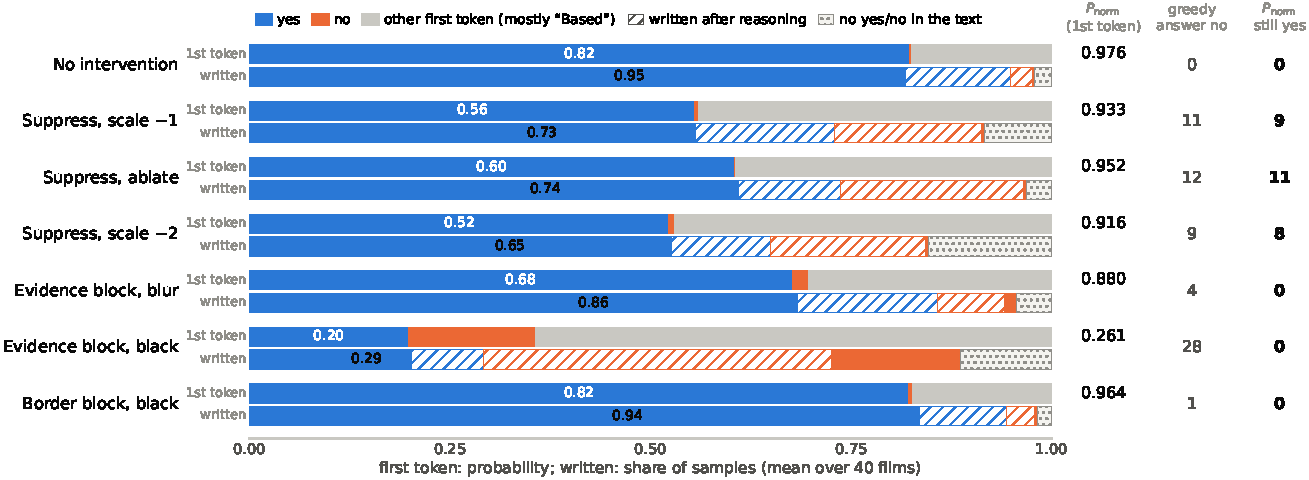
\includegraphics[width=0.96\textwidth]{fig1_split.pdf}
\caption{\textbf{What the first token says, and what the model then writes.} For each intervention,
the upper bar splits the probability of the first output token into ``yes'' (blue, $\Praw$), ``no''
(orange) and every other token (grey, mostly ``Based''); $\Pnorm$, printed at right, is blue
over blue plus orange. The lower bar splits sampled answers by what they conclude and how: solid
segments answer directly, hatched segments reason first, and dotted segments give neither answer.
Suppression moves the first token from ``yes'' to reasoning, and the reasoning now often concludes
``no'', which $\Pnorm$ misses. Right: films whose greedy answer is no, and among them those on which
$\Pnorm$ still says yes. The evidence block is the image region whose occlusion most lowers the
first-token readout, the border block a control at the image edge (\S\ref{sec:evidence};
Table~\ref{tab:main} adds a third occlusion, mean fill). Means over \val{n.fp} cardiomegaly false
positives (labelled negative, called positive), \val{e4.nsamples} samples each.}
\label{fig:split}
\end{figure}

We test this in a medical VLM. We steer MedGemma 1.5 by suppressing features of a transcoder, a
learned dictionary that rewrites the model's internal activations as sparse, more interpretable
features, and compare three first-token readouts with the answers the model writes, greedily and
when sampled. On one radiograph the normalized probability of ``yes'' after suppression is
\val{ex.norm}, and the model writes ``\textit{Based on the image, the chest X-ray shows a normal heart
size}'' before answering no (\S\ref{sec:clamp}). As a reference, we occlude the region of the
radiograph that the call depends on, an intervention whose effect the readouts should register;
because that region is found with a first-token readout, the reference favours the readout.
Figure~\ref{fig:split} shows the result. We then ask what the gap depends on. We apply the edit as a
\emph{clamp}, following the constrained patching of circuit tracing \citep{ameisen2025circuit}:
throughout the prompt, the outputs of the feed-forward (MLP) blocks are held at their unedited values
plus the edit's change. The first answer token is predicted at the last prompt position, whose MLP
blocks therefore cannot respond to the edit; every later token is predicted at a new position, whose
blocks can. So we also apply the edit to the \emph{live model}, in which every block responds. The gap
we report is measured under the clamp, the setting of circuit-tracing tools. Every verdict below comes from a
decision rule committed before its run; post hoc comparisons are marked~\dag.

\paragraph{Contributions.}
\begin{enumerate}\itemsep2pt
\item \textbf{A dissociation.} Suppressing the $80$ most active image features changes the model's
written answers, while the normalized readout still says yes on \val{pf.clamp.gnoyes} of the
\val{pf.clamp.gno} greedy answers that turn to ``no'' (\val{pf.occ.gnoyes} of \val{pf.occ.gno} when
the evidence is occluded instead\dag). It holds on radiographs that no first-token readout selected
(\S\ref{sec:clamp}).
\item \textbf{Two routes, and the clamp as a candidate cause.} Suppression shifts answers from
``Yes'' at once to reasoning first, and makes the reasoning end in ``no'' more often. The raw
probability of ``yes'' registers the shift but counts every reasoned answer as not-yes; the
normalized one registers neither (\S\ref{sec:routes}). We hypothesize that the first token stays at
``yes'' because the clamp holds the MLP blocks at the answer position fixed: applied to the live
model, the edit moves the first token with the answers, though only as a stronger edit and too
imprecisely to confirm (\S\ref{sec:live}).
\item \textbf{Where else it holds.} The dissociation recurs on correct calls of effusion and
pneumothorax. On correct cardiomegaly calls suppression barely changes the answers, so the test of
whether it generalises is inconclusive, and with non-answers set aside it finds that it does not.
Without an intervention, written answers and readouts rank radiographs alike in CheXagent-2, a VLM
that answers at the first token; in MedGemma the test cannot rule out a difference
(\S\ref{sec:scope}).
\item \textbf{Why the suppression is not finding-specific.} Selecting the most active features picks
nearly the same set for every finding; contrast between positive and negative radiographs gives
finding-specific sets, whose suppression barely changes the answers
(\S\ref{sec:selection}).
\end{enumerate}
We release the transcoder (\val{clt.used}B trained parameters), the code, and a result file behind every
number.\footnote{Code and results: \url{https://github.com/kevinjin918/first-token-readouts}.
Transcoder: \url{https://huggingface.co/kevinjin918/medgemma-1.5-cxr-clt}.}

\paragraph{Scope.} One steered model, one dataset and one family of interventions, applied in two
ways, with tens of radiographs per group. We show that a recommended readout can miss an
intervention's effect in a realistic medical setting, and by what route, not how often published results are
affected.

\section{Setup}
\label{sec:setup}

\paragraph{Model, data and prompt.} We steer MedGemma 1.5-4b-it \citep{medgemma2026,medgemma2025}
in bfloat16 on a $4{,}999$-image subset of NIH ChestX-ray14 \citep{wang2017chestxray} ($1{,}335$
patients). Each radiograph is presented in a single turn with the question ``Does this chest X-ray
show \textit{finding}? Answer yes or no.'' ChestX-ray14 labels are mined from radiology reports and
are noisy; we use them only to select radiographs, and every steering comparison compares the model
with itself.

\paragraph{First-token readouts.} Let $\ell$ be the logits at the position where the answer would
begin and $p = \operatorname{softmax}(\ell)$. Taking the largest logit among the first tokens of the
surface forms of each answer (\say{yes}, \say{\textvisiblespace yes}, \say{Yes},
\say{\textvisiblespace Yes}, \say{YES}, and the same for ``no''), we define
\[
\Praw = p_{\text{yes}}, \qquad
m = p_{\text{yes}} + p_{\text{no}}, \qquad
\Pnorm = \frac{p_{\text{yes}}}{p_{\text{yes}} + p_{\text{no}}} = \sigma(\Delta), \quad
\Delta = \ell_{\text{yes}} - \ell_{\text{no}}.
\]
$\Praw$ is the probability that the next token is ``yes''. The answer mass $m$ approximates the
probability that the next token is an answer at all. $\Pnorm$, a sigmoid of the yes-minus-no logit margin
$\Delta$, is the probability-scale form of the logit difference recommended for activation
patching \citep{zhang2024patching,heimersheim2024patching}. The three satisfy $\Praw = \Pnorm\cdot m$.
$\Pnorm$ saturates near $1$ on the radiographs below (median baseline $\Delta$ of
\val{fp.base.gapmedian} nats, odds of about \val{fp.base.gapodds} to $1$ for ``yes'' over ``no''), so
we also report $\Delta$ and the number of films on which each readout is below $0.5$.

\paragraph{Written answers.} For each radiograph and intervention we decode greedily and draw
\val{e4.nsamples} samples at temperature $1$ (no top-$k$ or nucleus truncation), up to
\val{e4.maxtok} new tokens. A fixed rule
parses each text: remove markdown symbols, lowercase, and take the first whole word ``yes'' or
``no''; if there is none, the text gives neither answer. The \emph{sampled yes rate} $s$ is the
fraction of samples that say yes. A sample \emph{answers directly} if its first word is ``yes'' or
``no'' and \emph{reasons first} otherwise. A blind hand reading agreed with the rule on
\val{hand.e4.agree} of \val{hand.e4.n} random samples. The rule errs toward ``neither'', and counting
such answers as yes or as no changes no conclusion below
(Appendix~\ref{app:parse}).

\paragraph{The steering intervention.} A cross-layer transcoder (CLT) reads the input to each MLP
block and reconstructs the outputs of that block and all later ones from a sparse set of
features \citep{lindsey2024crosscoders,ameisen2025circuit}. Ours covers all $34$ layers with $2{,}048$
features per layer and was trained on activations from radiographs and, separately, report texts
(Appendix~\ref{app:instrument}). We pick the $80$ features with the highest mean activation over
the radiograph's image tokens and edit them there: \texttt{scale}~$\lambda$ multiplies a feature's
activation by $\lambda$ ($\lambda=-1$ reverses its sign, $\lambda=-2$ reverses and doubles it) and
\texttt{ablate} sets it to zero. To apply an edit, we run the unedited prompt once and record, at
every prompt position and layer, the transcoder's feature activations and its reconstruction error,
the error term of \citet{ameisen2025circuit}. We then rerun the prompt with each MLP output replaced
by the reconstruction from the recorded features, edited at image positions, plus the recorded
error. With no edit this is the original output; with an edit, each MLP output in the prompt equals
its unedited value plus the decoded change and is not recomputed from its changed input, while
attention is recomputed throughout. We call this the \emph{clamp}. Every first-token readout reads
the logits at the last prompt position, a text position whose MLP outputs therefore keep their
unedited values, so the edit reaches those logits only through attention. Each later token is
predicted at a new position by the model's own MLP blocks, which respond to the edit as they attend
to the clamped prompt. Constrained patching \citep{ameisen2025circuit} holds a range of layers and
freezes attention patterns, but shares with the clamp the property our hypothesis concerns: MLP
blocks at the readout position cannot respond to the edit. The generation function of the circuit-tracer library
\citep{hanna2025circuittracer} likewise applies its constraints only while predicting the first new
token.\footnote{The documentation of \texttt{feature\_intervention\_generate} states that the
constraints ``will only apply to the very first token generated''; later tokens attend to the cached
states of the constrained pass.} \S\ref{sec:live} instead edits the live model. The first generated
token has the readouts' distribution
(Appendix~\ref{app:repro}).

\paragraph{Radiographs.} The main comparison uses radiographs (\emph{films}) that the model calls
positive for cardiomegaly although ChestX-ray14 labels them negative (false positives with respect to the label), all
anteroposterior (AP). AP projection
magnifies the cardiac silhouette relative to the standard posteroanterior view, so the heart can look
enlarged when it is not. Chest-radiograph classifiers are known to pick up how a film was acquired:
whether it was taken with a portable X-ray unit \citep{zech2018} and, probably, its projection
\citep{degrave2021}. On these films the model's call plausibly depends on the heart's
apparent size, which makes the location of the evidence checkable; the reference below does not
require the call to be right or wrong. The \val{n.fp} films, from \val{n.fppatients} patients, form
two sets of \val{n.fpbanked} with no patient in both. The first, from the pilot study behind this paper's
submitted version, was selected by $\Praw \geq 0.5$. The second, drawn for this paper, was selected by
the model's greedy answer being yes, so that no readout under test chose it
(Appendix~\ref{app:sets}). For correct calls and other findings we drew \val{n.tpcardiomegaly}
radiographs each for cardiomegaly, pleural effusion (fluid around the lung) and pneumothorax (air
around the lung), labelled positive and answered yes by the greedy answer, one per patient and no patient in two sets.

\paragraph{Pre-registration.} Every test we call pre-registered had its decision rule and thresholds
committed in its script before the run. The text states outcomes in plain words, with the rule's
label in small capitals; Appendix~\ref{app:rules} gives each rule, its outcome and every amendment.
Post hoc comparisons are marked~\dag.

\section{A reference effect: occluding the evidence}
\label{sec:evidence}

\begin{figure}[t]
\centering
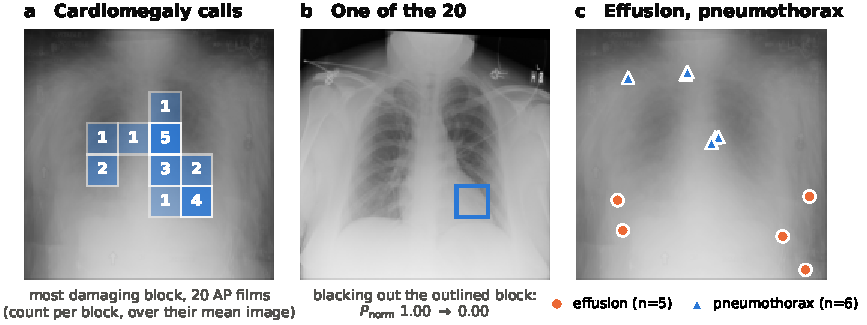
\includegraphics[width=0.92\textwidth]{fig_location.pdf}
\caption{\textbf{Where the evidence for each call sits.} \textbf{(a)} For each of the first \val{loc.n}
false-positive radiographs, the $2\times2$-token block whose black occlusion most lowers $\Praw$,
counted on the $8\times8$ block grid and drawn over the mean of the \val{loc.n} images. All \val{loc.central} fall over
the cardiac silhouette and the mediastinum. \textbf{(b)} One of the \val{loc.n}: blacking out the outlined
block, at the left heart border, takes $\Pnorm$ from \val{loc.ex.base} to \val{loc.ex.black}. \textbf{(c)} The most
damaging block on a separate set of \val{attn.tpeff.n} effusion- and \val{attn.tpptx.n}
pneumothorax-positive radiographs, which may include several films per patient
(Appendix~\ref{app:attention}), for films
where one block moves $\Pnorm$ by more than $0.15$. Effusion blocks lie at the lung bases; pneumothorax blocks lie in the
upper zones or, on three films from one patient, over a chest tube.}
\label{fig:location}
\end{figure}

To know what a readout should register, we need an intervention that changes the call through its
evidence. MedGemma encodes each image as a $16\times16$ grid of tokens. We occlude one $2\times2$
block of that grid (one sixty-fourth of the image) at a time and record the change in the first-token
readout. The block with
the largest effect is the film's \emph{evidence block}\footnote{For the first \val{loc.n} films, the block
that most lowers $\Praw$, as chosen in the pilot study; for films drawn for this paper, the block
that most lowers $\Delta$.}. On \val{loc.central} of the first \val{loc.n} false-positive films it
lies in the central $4\times4$ blocks, and on \val{loc.leftheart} in the two columns just right of
the image midline, the patient's
left, where most of the cardiac silhouette lies (Figure~\ref{fig:location}a,b). The same procedure on
other findings gives locations that match their radiographic appearance (Figure~\ref{fig:location}c):
lung bases for effusion, upper zones for pneumothorax, and on one patient the curled tip of a chest
tube, the treatment-device shortcut documented by \citet{oakdenrayner2020}. On the false positives,
then, the evidence block lies on the cardiac silhouette, whose apparent size depends on the
projection, rather than on a finding the label records; on correct calls it lies where the finding
appears or, for one patient, on a chest tube. These descriptions are our own; no radiologist reviewed them.

Occlusion is our reference for an intervention that changes the call, and the first-token readouts
follow it (Table~\ref{tab:main}, lower rows). Blacking out the evidence block turns the greedy answer
to ``no'' on \val{fp.black.greedyno} of \val{n.fp} films and lowers the sampled yes rate from
\val{fp.base.s} to \val{fp.black.s}; $\Pnorm$ says no on \val{fp.black.flipsnorm} films. Three
controls tie the effect to the evidence rather than to the occlusion. An identical black square at a
random border block leaves the answers in place, so the effect is not the size of the perturbation.
Mean fill, which leaves no high-contrast edge, still changes them, so it is not an edge artifact. And
on the \val{occ.eff.n} films of the first set also called positive for effusion, occluding the
cardiac block leaves that call at $\Pnorm \geq \val{occ.eff.minnorm}$, so it is not general damage to
the model. Applying the suppression's pre-registered rule to these rows\dag, no first-token readout
falls short of the answers when the evidence is removed; under suppression, $\Pnorm$ falls short by \val{fp.clamp.minshortfall} to
\val{fp.clamp.maxshortfall} (Table~\ref{tab:v1}).

\section{Feature suppression changes the written answer}
\label{sec:clamp}

\begin{table}[t]
\centering
\footnotesize
\setlength{\tabcolsep}{4pt}
% generated by paper/make_numbers.py; do not edit
\begin{tabular}{lcccccc}
\toprule
& \multicolumn{4}{c}{first token} & \multicolumn{2}{c}{written answer} \\
\cmidrule(lr){2-5}\cmidrule(lr){6-7}
Intervention & $\Praw$ & $\Pnorm$ & median $\Delta$ change & below $0.5$ & $s$ & greedy no \\
& & & (nats) & ($\Praw$ / $\Pnorm$) & & ($\Pnorm$ yes) \\
\midrule
None & 0.824 & 0.976 & -- & 5 / 1 & 0.95 & 0 (0) \\
Suppress, \texttt{scale} $-1$ & 0.555 & 0.933 & $-2.9$ & 16 / 2 & 0.73 & 11 (9) \\
Suppress, \texttt{ablate} & 0.604 & 0.952 & $-2.1$ & 14 / 1 & 0.74 & 12 (11) \\
Suppress, \texttt{scale} $-2$ & 0.523 & 0.916 & $-3.1$ & 17 / 3 & 0.65 & 9 (8) \\
\midrule
Evidence block, black & 0.198 & 0.261 & $-14.3$ & 31 / 31 & 0.29 & 28 (0) \\
Evidence block, mean fill & 0.296 & 0.469 & $-9.6$ & 28 / 21 & 0.44 & 21 (3) \\
Evidence block, blur & 0.677 & 0.880 & $-1.1$ & 12 / 5 & 0.86 & 4 (0) \\
Border block, black & 0.822 & 0.964 & $+0.0$ & 6 / 1 & 0.94 & 1 (0) \\
\bottomrule
\end{tabular}

\caption{\textbf{Suppression and occlusion on the same false-positive radiographs.} Means over
\val{n.fp} films. $\Delta$ is the yes-minus-no logit margin; ``below $0.5$'' counts films on which the
readout says no. $s$ is the fraction of sampled answers that say yes, and ``greedy no'' counts films whose
greedy answer is no; in parentheses, those on which $\Pnorm$ still says yes.}
\label{tab:main}
\end{table}

\begin{table}[t]
\centering
\footnotesize
\setlength{\tabcolsep}{3pt}
% generated by paper/make_numbers.py; do not edit
\begin{tabular}{lccccc}
\toprule
& & \multicolumn{2}{c}{$\Praw$} & \multicolumn{2}{c}{$\Pnorm$} \\
\cmidrule(lr){3-4}\cmidrule(lr){5-6}
Intervention & drop in $s$ & difference & verdict & difference & verdict \\
\midrule
\multicolumn{6}{l}{\emph{Suppression}} \\
\quad \texttt{scale} $-1$ & $0.22$ {\scriptsize[$0.16$,\,$0.28$]} & $+0.05$ {\scriptsize[$0.00$,\,$+0.09$]} & \textsc{unresolved} & $-0.18$ {\scriptsize[$-0.24$,\,$-0.12$]} & \textsc{misreads} \\
\quad \texttt{ablate} & $0.21$ {\scriptsize[$0.14$,\,$0.28$]} & $+0.01$ {\scriptsize[$-0.05$,\,$+0.06$]} & \textsc{unresolved} & $-0.19$ {\scriptsize[$-0.25$,\,$-0.13$]} & \textsc{misreads} \\
\quad \texttt{scale} $-2$ & $0.30$ {\scriptsize[$0.22$,\,$0.37$]} & $0.00$ {\scriptsize[$-0.04$,\,$+0.04$]} & \textsc{tracks} & $-0.24$ {\scriptsize[$-0.32$,\,$-0.16$]} & \textsc{misreads} \\
\multicolumn{6}{l}{\emph{Occlusion (reference)}} \\
\quad evidence, black & $0.66$ {\scriptsize[$0.54$,\,$0.76$]} & $-0.03$ {\scriptsize[$-0.09$,\,$+0.03$]} & \textsc{unresolved} & $+0.06$ {\scriptsize[$+0.03$,\,$+0.09$]} & \textsc{misreads} \\
\quad evidence, mean & $0.51$ {\scriptsize[$0.39$,\,$0.62$]} & $+0.02$ {\scriptsize[$-0.05$,\,$+0.10$]} & \textsc{unresolved} & $0.00$ {\scriptsize[$-0.05$,\,$+0.05$]} & \textsc{unresolved} \\
\quad evidence, blur & $0.09$ {\scriptsize[$0.03$,\,$0.17$]} & $+0.06$ {\scriptsize[$0.00$,\,$+0.11$]} & \textsc{misreads} & $+0.01$ {\scriptsize[$-0.02$,\,$+0.04$]} & \textsc{tracks} \\
\quad border, black & $0.01$ {\scriptsize[$-0.01$,\,$0.02$]} & $0.00$ {\scriptsize[$-0.02$,\,$+0.01$]} & \textsc{tracks} & $+0.01$ {\scriptsize[$0.00$,\,$+0.02$]} & \textsc{tracks} \\
\bottomrule
\end{tabular}

\caption{\textbf{Does a first-token readout fall by as much as the written answers?} Difference:
for each film, the readout's drop from the unedited model minus the drop in the sampled yes rate
$s$, negative when the readout falls by less than the answers, positive when by more. Mean over \val{n.fp} films with a $95\%$ film-bootstrap interval in brackets. Pre-registered verdicts:
\textsc{misreads} if the interval excludes $0$ and the mean exceeds $0.05$ in size, \textsc{tracks}
if the interval lies within $\pm0.05$, \textsc{unresolved} otherwise, computed before rounding. The rule was registered for
the suppression rows; the occlusion rows apply it as a reference, and their two \textsc{misreads}
cells are readouts that fall slightly further than the answers, as expected of a block chosen by a
first-token readout.}
\label{tab:v1}
\end{table}

\paragraph{What the first token says.} Read through $\Pnorm$, suppression leaves the model's call
nearly unchanged.\footnote{The submitted version of this paper drew this conclusion; the written
answers below overturn it.} We report \texttt{scale}~$-1$; \texttt{ablate} and \texttt{scale}~$-2$
agree throughout (Tables~\ref{tab:main} and~\ref{tab:v1}). Suppression lowers $\Praw$ from
\val{fp.base.raw2} to \val{fp.scale1.raw2}, but almost none of the lost probability goes to ``no''
(mean $p_{\text{no}} \leq \val{fp.clamp.pnomax}$ under every variant); it goes to ``Based''
(Figure~\ref{fig:split}). The margin $\Delta$ narrows but stays large, so $\Pnorm$ moves only from
\val{fp.base.norm} to \val{fp.scale1.norm} and says no on \val{fp.scale1.flipsnorm} of \val{n.fp}
films.

\paragraph{What the model writes.} The written answers tell a different story. On one film, under
\texttt{scale}~$-1$, $\Pnorm$ is \val{ex.norm} and the model writes:
\begin{quote}\small
\val{ex.clamp}
\end{quote}
Unedited, the same film gets ``\val{ex.base}'' The example is typical. Counting each film once per
variant, suppression turns \val{pf.clamp.gno} greedy answers to ``no'' (\val{fp.scale1.greedyno},
\val{fp.ablate.greedyno} and \val{fp.scale2.greedyno} under \texttt{scale}~$-1$, \texttt{ablate} and
\texttt{scale}~$-2$), on \val{pf.clamp.gnofilms} of the \val{n.fp} films, and $\Pnorm$ still says yes
on \val{pf.clamp.gnoyes} of them, each at $\Pnorm \geq \val{pf.clamp.missmin}$. The three occlusions
turn \val{pf.occ.gno} answers to ``no'', and $\Pnorm$ misses \val{pf.occ.gnoyes}\dag, a comparison
that favours the readout, since the evidence blocks were chosen with a first-token readout
(Table~\ref{tab:main}).

Sampled answers show the same gap, and the pre-registered tests confirm it. A first check on
\val{e2.n} films had a pre-registered rule: $\Pnorm$ misses the effect if suppression turns the greedy answer to
``no'' on at least $3$ films where $\Pnorm$ still says yes. It did, under all three variants. In the
replication (\val{n.fp} films, \val{e4.nsamples} samples each), \texttt{scale}~$-1$ lowers the
sampled yes rate from \val{fp.base.s} to \val{fp.scale1.s}, and under each variant $\Pnorm$ falls
short of the drop in $s$ by \val{fp.clamp.minshortfall} to \val{fp.clamp.maxshortfall}
(Table~\ref{tab:v1}).
The rule calls this a miss under all three (\textsc{misreads}). On the \val{n.fpfresh} films chosen by
greedy answer alone, which no first-token readout selected, the first check's rule is met again
(\val{v.V2}), and the verdicts hold with non-answers set aside. Per-film effects are
sensitive to near-ties at the top-$80$ cutoff (Appendix~\ref{app:repro}), so we report means and
pooled counts.

\subsection{Two routes to the answer}
\label{sec:routes}

\begin{table}[t]
\centering
\footnotesize
% generated by paper/make_numbers.py; do not edit
\begin{tabular}{lcccc}
\toprule
& \multicolumn{2}{c}{answers directly} & \multicolumn{2}{c}{reasons first} \\
\cmidrule(lr){2-3}\cmidrule(lr){4-5}
Intervention & share & says yes & share & says yes / no / neither \\
\midrule
None & 0.82 & 1.00 & 0.18 & 0.73 / 0.16 / 0.12 \\
Suppress, \texttt{scale} $-1$ & 0.56 & 0.99 & 0.44 & 0.39 / 0.42 / 0.19 \\
Suppress, \texttt{ablate} & 0.61 & 0.99 & 0.39 & 0.33 / 0.59 / 0.08 \\
Suppress, \texttt{scale} $-2$ & 0.53 & 0.99 & 0.47 & 0.26 / 0.41 / 0.33 \\
Evidence block, black & 0.36 & 0.56 & 0.64 & 0.14 / 0.68 / 0.18 \\
\bottomrule
\end{tabular}

\caption{\textbf{Sampled answers by their first word,} pooled over \val{n.fp} films and
\val{e4.nsamples} samples each. Answers that open with ``Yes'' or ``No'' give that answer by
construction. Suppression moves answers to the reasoning route and changes where that route
ends.}
\label{tab:routes}
\end{table}

Why does the text move when $\Pnorm$ barely does? Sampled answers fall into two groups by their first
word (Table~\ref{tab:routes}). Some open with ``Yes'' or ``No'' and answer at once; almost all of
these say yes. The rest, almost always opening ``Based on the image'', reason first. Write $r$ for the
share of samples that reason first and $y$ for the share of those that conclude yes. Since a sample
opens with ``Yes'' with probability about $\Praw$,
\[
s \;\approx\; \Praw + r\,y .
\]
Suppression changes both terms. It moves first-token probability from ``Yes'' to ``Based'' (from
\val{fp.base.based} to \val{fp.scale1.based}), which lowers $\Praw$ and raises $r$ from
\val{route.base.reasoned} to \val{route.scale1.reasoned}, and it lowers $y$ from
\val{route.base.ryes} to \val{route.scale1.ryes}. $\Pnorm$ compares ``yes'' with ``no'' at the first
token, where ``no'' is almost never chosen, so it registers neither change: depending on the
variant, it falls by less than $0.01$ on \val{ceil.tinymin} to \val{ceil.tinymax} of the \val{n.fp}
films, while on those films $s$ falls by \val{ceil.sdroptinymin} to \val{ceil.sdroptinymax} on
average. The margin $\Delta$ does register the suppression: its median change orders all seven
interventions as the drop in $s$ does (Table~\ref{tab:main})\dag. But from a median of
\val{fp.base.gapmedian} nats it rarely crosses zero, because the lost ``yes'' probability goes to
``Based'', which the margin leaves out, not to ``no''. The miss is therefore not only the saturation
of the sigmoid: on the margin's own scale the first token still strongly prefers ``yes'' to ``no''
while the written answers turn to no.

$\Praw$ falls by about as much as $s$ (\val{fp.scale1.rawdrop} against \val{fp.scale1.sdrop}), but by
coincidence. It is the first term alone, so $s - \Praw \approx r\,y$, and suppression leaves $r\,y$
nearly unchanged (\val{route.base.ryesall} unedited, \val{route.scale1.ryesall} under
\texttt{scale}~$-1$): it raises $r$ while lowering $y$. The two changes happen to cancel on these films. By the pre-registered rule $\Praw$ tracks the answers under one
variant and is unresolved under the other two, and with answers that give neither set aside it
overstates the effect under two (Table~\ref{tab:v1}, Appendix~\ref{app:rules}).

\subsection{Is the clamp the cause? Applying the edit to the live model}
\label{sec:live}

If holding the answer position's MLP blocks fixed is why the first token misses what the reasoning
concludes, applying the edit to the live model, where every block responds, should move the first
token with the answers. Strength alone does not close the gap under the clamp: under
\texttt{scale}~$-2$, $s$ falls by \val{fp.scale2.sdrop} and $\Pnorm$ only to \val{fp.scale2.norm}. In
two pre-registered tests on the same \val{e8.nfilms} films, feature sets and seeds, we added each
edit's change in the transcoder's output to the model's own MLP outputs (Appendix~\ref{app:live}). At
the strengths of \S\ref{sec:clamp} the live edit is far stronger than the clamp:
\val{e8.none.min} to \val{e8.none.max} of samples give neither answer. $\Pnorm$ then falls by less
than $s$ under two variants but by more than the yes rate among answering samples under all three
(\val{e8.verdict}), so neither comparison is clean. The second test weakened the edit, scaling each
feature by $\lambda$ from $0.9$ down to $0.15$ ($\lambda = 0.6$ removes $40\%$
of each activation, a fifth of the change that \texttt{scale}~$-1$ makes). A strength counted only if
it still lowered $s$ (interval above $0.05$) and at most \val{e9.tau} of samples failed to answer, the
most under any intervention of the replication. The response is a cliff ($s$ falls by
\val{e9.weak.sdrop} at $\lambda = \val{e9.weak.c}$ and by \val{e9.sdrop} at $\lambda = 0.6$), so only
$\lambda = 0.6$ qualified. There the first token moves with the answers: it puts probability
\val{e9.pno} on ``no'', against at most \val{fp.clamp.pnomax} under the clamp, and $\Pnorm$ and $s$
fall by about the same amount (difference \val{e9.normvs}).

This is consistent with the clamp as the cause of the dissociation but does not establish it, for
three reasons. (i)~Dose: the eligible strength changes the answers \val{e9.ratio} times as much as the
clamp, and no live strength as mild as the clamp still changed them, so the two are never compared
at a matched effect. (ii)~Precision: the interval is wider than the $\pm0.05$ the rule needs to call
agreement (\val{e9.verdict}). (iii)~Confound: the live edit lets the MLP blocks at image positions
respond as well as those at the answer position, so it does not isolate the condition we
hypothesize; freeing only the answer position's blocks would, and we did not run it.

\section{Beyond the false positives}
\label{sec:scope}

\paragraph{Correct calls and other findings.} The false-positive films are one population. On
correctly called films the gap reappears for effusion and pneumothorax, while cardiomegaly calls
barely respond to suppression (Table~\ref{tab:tp}). We repeated \texttt{scale}~$-1$ and the evidence
occlusion on \val{n.tpcardiomegaly} correctly called positive films for each of three findings.
Suppression lowers $s$ by \val{tpeffusion.scale1.sdrop} for effusion and
\val{tppneumothorax.scale1.sdrop} for pneumothorax, and by the pre-registered rule $\Pnorm$ misses
the effect on both (\textsc{misreads}), as on the false positives. For cardiomegaly $s$ falls by
only \val{tpcardiomegaly.scale1.sdrop}, too little for the rule to separate $\Pnorm$ from the answers,
so the verdict on whether the dissociation generalises is \val{v.V3s}; with non-answers set aside,
$\Pnorm$ tracks the answers on cardiomegaly, and by the rule the dissociation \val{v.V3c}. We read
this\dag\ as an edit too weak on these calls for any readout to miss: blacking out the evidence block
moves them ($s$ falls by \val{tpcardiomegaly.black.sdrop}), but this suppression hardly does.

\begin{table}[t]
\centering
\footnotesize
\setlength{\tabcolsep}{3pt}
% generated by paper/make_numbers.py; do not edit
\begin{tabular}{lccccccc}
\toprule
& \multicolumn{3}{c}{no intervention} & \multicolumn{3}{c}{suppression, \texttt{scale} $-1$} & evidence black \\
\cmidrule(lr){2-4}\cmidrule(lr){5-7}\cmidrule(lr){8-8}
Finding & $\Praw$ & $m$ & $s$ & drop in $s$ & difference, $\Praw$ & difference, $\Pnorm$ & drop in $s$ \\
\midrule
Cardiomegaly & 0.97 & 0.97 & 0.99 & $0.04$ {\scriptsize[$0.02$,\,$0.07$]} & $+0.04$ {\scriptsize[$+0.02$,\,$+0.06$]} & $-0.04$ {\scriptsize[$-0.07$,\,$-0.01$]} & $0.28$ {\scriptsize[$0.11$,\,$0.48$]} \\
Effusion & 0.92 & 0.92 & 0.96 & $0.17$ {\scriptsize[$0.07$,\,$0.28$]} & $+0.02$ {\scriptsize[$-0.01$,\,$+0.05$]} & $-0.15$ {\scriptsize[$-0.26$,\,$-0.05$]} & $0.22$ {\scriptsize[$0.07$,\,$0.37$]} \\
Pneumothorax & 0.91 & 0.93 & 0.96 & $0.21$ {\scriptsize[$0.11$,\,$0.32$]} & $+0.02$ {\scriptsize[$-0.01$,\,$+0.05$]} & $-0.16$ {\scriptsize[$-0.24$,\,$-0.08$]} & $0.29$ {\scriptsize[$0.13$,\,$0.47$]} \\
\bottomrule
\end{tabular}

\caption{\textbf{Correctly called radiographs, three findings.} \val{n.tpcardiomegaly} per finding,
labelled positive and answered yes. Difference: the readout's drop minus the drop in $s$, as in
Table~\ref{tab:v1}; mean with $95\%$ film-bootstrap interval. Pre-registered verdicts for
$\Pnorm$: \val{tpcardiomegaly.scale1.normvs.v} for cardiomegaly, \val{tpeffusion.scale1.normvs.v} for
effusion and \val{tppneumothorax.scale1.normvs.v} for pneumothorax; for $\Praw$,
\val{tpcardiomegaly.scale1.rawvs.v} on all three.}
\label{tab:tp}
\end{table}

\paragraph{Evaluation without an intervention.} Does the choice of readout also matter when nothing
is edited? A pre-registered test on \val{e7.npat} patients not used elsewhere asked whether one
ordinary closed evaluation, \val{e7.nper} positive and \val{e7.nper} negative films per finding, ranks
films differently when scored by a first-token readout or by the written answers, measured as AUC
against the label. To compare scores of equal coarseness, each readout $P$ is scored as the yes rate
of \val{e7.nsamples} simulated answers drawn at probability $P$ (Appendix~\ref{app:e6}). In CheXagent-2
3B \citep{chexagent2024}, a chest-radiograph VLM that answers at the first token, the two scores rank
films alike. In MedGemma, whose answer mass on these films is only \val{e7.mg.massmin} to
\val{e7.mg.massmax}, the test detects no difference in AUC (at most \val{e7.maxabsD}) but cannot
exclude one up to \val{e7.mg.maxbound} (\val{e7.mg.verdict}). Per film, MedGemma's yes counts depart
from the readout more often than chance\dag. An earlier test did find a difference, but it compared
the continuous readout with $s$ directly, and that difference is an artifact of their different
resolution (Appendix~\ref{app:e6}). The dissociation of \S\ref{sec:clamp} differs in kind: $\Pnorm$
misses most of a change in the answers.

\section{Why the suppression is not finding-specific}
\label{sec:selection}

The suppression changes the answers, but not specifically for cardiomegaly, so
\S\ref{sec:clamp} shows a readout failing under a generic perturbation of image features, not under
removal of cardiomegaly evidence.

\paragraph{Top-activation selection is finding-agnostic.} If the $80$ most active image features were
the model's cardiomegaly evidence, the same rule applied to radiographs with other findings would
pick different features. We built feature sets by this rule from \val{e3.ndonor} \emph{donor} radiographs, used only to
choose features, for each of
cardiomegaly, effusion and pneumothorax, one radiograph per patient and no patient shared across
sets or with the test films. The sets overlap almost completely: mean pairwise Jaccard
\val{e3.jac.activation.80} at $N{=}80$, against \val{e3.jac.contrast.80} when features are selected by their
contrast between positive and negative donors (Table~\ref{tab:jaccard} in
Appendix~\ref{app:donors}). Top activation
picks the image features most active on any chest radiograph.

\paragraph{Does selecting by contrast help?} With larger donor groups, we selected the $80$ features
whose mean activation differs most between \val{e5.ndonor} positive and \val{e5.ndonor} negative
radiographs, one set for cardiomegaly and one for effusion (Jaccard \val{e5.jaccon}), with no patient
shared with the test films or across sets. They share on average \val{e5.fp.concard.overlap} of their
$80$ features with each film's top set, and suppressing them barely changes the answers. On correct
calls of its own finding neither set beats $80$ randomly drawn active features by the pre-registered
margin, nor does the cardiomegaly set on the false positives (Table~\ref{tab:e5} in
Appendix~\ref{app:tables}). The features that separate positive from negative
radiographs are not the ones whose suppression moves the answer, although we did not record how
strongly they fire on the test films.

\section{Related work}
\label{sec:related}

\paragraph{First-token readouts of interventions.} Activation steering of the live MedGemma has been scored from the
next-token ``Yes'' and ``No'' logits without parsing the text, noting that steering changes their
combined mass \citep{farina2026steering}, and
sparse-autoencoder patching of MedGemma from the yes-minus-no margin \citep{sadanandan2026b}.

\paragraph{The choice of metric.} \citet{zhang2024patching} show that probability and logit
difference can lead to different conclusions in activation patching and recommend the logit
difference; \citet{heimersheim2024patching} note that it is insensitive to components that move all
the compared logits together, which is the blind spot we measure. Steering work on multiple-choice
questions uses the probability normalized over the two options (in the released code of
\citealp{rimsky2024caa}) or the logit difference \citep{tan2024steering}; \citet{tan2024steering}
argue that the model decides at the answer token, and our result is a case where it does not.
Steering vectors built from multiple-choice questions can fail on open-ended answers
\citep{pres2024reliable}, and model edits look far stronger under teacher forcing than in free
generation \citep{yang2025mirage}. \citet{arditi2024refusal} use a first-token proxy for refusal
and note that full completions are more accurate. \citet{lindsey2025biology} report a circuit-tracing
intervention whose outcome reverses when attention is allowed to respond. We add a same-prompt case where the first-token readout and the
generated answer disagree, the routes by which they part, and a candidate condition: a first token computed
under constraints that the rest of the answer is not.

\paragraph{First tokens and generated text without intervention.} Instruction-tuned models shown
the options place nearly all first-token probability on them \citep{wiegreffe2023mass}; MedGemma,
told to answer yes or no, often does not. First-token probabilities often disagree with generated answers
\citep{wang2024answerc,lyu2024beyond}, though under image swaps in MedGemma-27B they agree on $91$
to $99\%$ of cases \citep{cajas2026modalens}. Generated answers are the more robust of the two to question
perturbations \citep{wang2024lookattext}. Alternative first tokens open reasoning paths that
change the answer \citep{wang2024cotdecoding}, and steering can induce such reasoning
\citep{zhang2024steeringcot}, including through sparse-autoencoder features \citep{he2026triggering}.
In medical VLMs, \citet{nooralahzadeh2026universal} steer with sparse-autoencoder features and
evaluate generated reports.

\section{Discussion}
\label{sec:discussion}

\paragraph{Recommendation.} When an intervention is evaluated on a closed question, score sampled
answers, and report the first-token readouts and the share of answers that reason first alongside
them. Scoring the answers would have caught both failures we saw: a first token that misses what
the reasoning concludes under the clamp, and a readout that still reports a decision when strong live
edits stop the model from answering. A harness that constrains only the pass that predicts the
first token, as our clamp and circuit-tracer's generation function do, reads the first token and the
rest of the answer from differently constrained computations; whether that caused the gap here is
open (\S\ref{sec:live}), but both should come from one configuration, or be labelled. A fall in the
answer mass $m$ shows that the first token no longer carries most answers, not which way they moved:
$m$ fell further under black occlusion (\val{fp.black.mass}), where $\Pnorm$ followed the answers,
than under suppression (\val{fp.scale1.mass}). A greedy answer alone can hide a shift in the
distribution \citep{pres2024reliable}; \val{e4.nsamples} samples per film sufficed here.

\paragraph{What we do not claim.} We do not claim the logit difference is a bad metric. When the model
answers at the first token ($m$ near $1$) it describes the decision and is the right tool for the
patching studies it was recommended for. Here, where the model often does not, the margin still
ranked the interventions as the answers did\dag, but could not say what the model then answered. We do not claim that first-token readouts fail however an
edit is applied: under the live edit $\Pnorm$ followed the answers on average, though too imprecisely to confirm agreement. We do not claim that published steering results are wrong;
we measured one model and one dictionary. We do not claim the model's cardiomegaly calls on these
films are clinically right or wrong, and we do not read the generated reasoning as an explanation of
the model's computation \citep{lanham2023faithfulness,cox2026precommit}.

\paragraph{Limitations.} One steered model and one dataset, with \val{n.fp} false-positive and
\val{n.tp} true-positive radiographs in the steering comparisons, and \val{e3.ndonor} donor
radiographs per feature set. No radiologist reviewed the radiographs, the labels, the occlusion maps or the generated text,
and the anatomical descriptions are our own. ChestX-ray14 labels are mined from reports and noisy.
The parse rule reads the first ``yes'' or ``no'' within \val{e4.maxtok} tokens, and a model could
revise its answer later. The hand reading was done by the author, blind but not independent; no second
reader checked it. Sampling at temperature $1$
without truncation is not how a deployed model decodes, but the greedy answers tell the same story. The live-edit test rests on one strength, with \val{e9.ratio}
times the clamp's effect.

\begin{ack}
Compute for this work was provided by the YC Summer Fellowship. The author declares no
competing interests.
\end{ack}

\bibliographystyle{plainnat}
\bibliography{references}

\clearpage
\appendix

\section{Pre-registered decision rules}
\label{app:rules}

Each rule was written into the experiment's script and committed to the repository before the run;
the commit hashes are in the result files. Results are stated in the rule's own terms.

\begin{itemize}\itemsep3pt
\item \textbf{Generation check} (first check, $20$ films, $10$ samples). Per suppression variant:
\textsc{disagrees} if the greedy answer is ``no'' on at least $3$ films where $\Pnorm$ calls yes;
otherwise \textsc{hedge-dominated} if it gives neither answer on at least $5$; otherwise
\textsc{validated} if it matches the $\Pnorm$ call on at least $18$; otherwise \textsc{mixed}.
Result: \textsc{disagrees} for all three variants (\val{e2.scale1.greedyno}, \val{e2.ablate.greedyno}
and \val{e2.scale2.greedyno} films under \texttt{scale}~$-1$, \texttt{ablate} and \texttt{scale}~$-2$).
The script first required the unedited model
and \texttt{scale}~$-1$ to reproduce the pilot study's $\Praw$ within $0.02$ on every film, or the
run would stop. It was amended twice; neither amendment changed the films, arms, seed or verdict
rules. When \texttt{scale}~$-1$ failed on two of the first five films, because a feature at the
top-$80$ boundary had swapped on the new software stack (Appendix~\ref{app:repro}), the requirement
was kept for the unedited model only; this was committed before any generated text was read. When
the unedited model's $\Praw$ then drifted by \val{e2.base.banked} on the seventh film, the
requirement was dropped and the drift reported, and the run restarted from the first film. This
second amendment was not blind: the parsed greedy answers for the first six films had been seen.
\item \textbf{Replication with sampled answers} (\val{n.fp} false-positive films,
\val{e4.nsamples} samples). For each
suppression variant, the per-film difference between a readout's change and the change in $s$ is
bootstrapped ($10{,}000$ resamples). \textsc{misreads} if the $95\%$ interval excludes $0$ and the
mean exceeds $0.05$ in size; \textsc{tracks} if the interval lies within $\pm0.05$; otherwise
\textsc{unresolved}. $\Pnorm$ is \textsc{supported} as missing the effect if all three variants
misread, \textsc{refuted} if all three track, and \textsc{partial} otherwise; likewise $\Praw$. Fresh films: the first check's rule, \textsc{replicates} if at least $2$ of $3$ variants
disagree. True positives, under \texttt{scale}~$-1$: a finding shows an effect if the interval of
its drop in $s$ excludes $0$; \textsc{generalises} if at least two findings show an effect and
$\Pnorm$ misreads on all of them, \textsc{does not generalise} if $\Pnorm$ tracks on any of them,
otherwise \textsc{inconclusive}. Every verdict is repeated with $s$ computed over answered samples
only. Results: $\Pnorm$ \val{v.V1norms} and $\Praw$ \val{v.V1raws} as missing the effect
(answered samples only: \val{v.V1normc}, \val{v.V1rawc}); fresh films \val{v.V2}; true positives
\val{v.V3s} (answered only: \val{v.V3c}).
\item \textbf{Contrastive selection} (\val{n.fp} false positives and \val{n.tpcardiomegaly}
correctly called films each for cardiomegaly and effusion). Every set has $80$ features and is
suppressed with \texttt{scale}~$-1$; $d$ is a film's drop in $s$, with $10{,}000$-resample film
bootstrap intervals. Specificity: \textsc{selection rescues specificity} if, on correct cardiomegaly
calls, the cardiomegaly contrast set lowers $s$ by more than the effusion set (mean above $0.10$,
interval above $0$) and the converse holds on correct effusion calls; \textsc{contrastive sets
inert} if neither contrast set beats random active features by $0.10$ (upper bound) on its own
finding; otherwise \textsc{mixed}. On the false positives, cardiomegaly contrast against random
active features, and evidence-block against border-block anchoring, each judged at the same $0.10$
threshold; the anchoring difference is also reported, without a verdict, on each group of correct
calls. Results: specificity \val{e5.S1}; on the false positives \val{e5.S2} and, for anchoring,
\val{e5.S3}.
\item \textbf{Evaluation} (\val{e6.npairs} radiograph--finding pairs, \val{e6.mg.nsamples} samples
each). AUC against the label under each score, with $2{,}000$-resample paired film-bootstrap
intervals. Per model, over the six differences between a first-token readout's AUC and that of
$s$: \textsc{readout changes the evaluation} if some difference exceeds $0.03$ in size with an
interval excluding $0$; \textsc{innocuous} if every interval lies within $\pm0.03$; otherwise
\textsc{unresolved}. Across the two models, per finding: \textsc{ranking reverses} if a first-token
readout and $s$ each separate the models in opposite directions; \textsc{ranking differs in
significance} if exactly one of them separates the models; otherwise \textsc{same ranking}. Two
amendments concern the second model only. The first, before any second-model run, replaced
Lingshu-7B with CheXagent-2 3B and fixed its prompt to the model card's format with a newline
appended after the assistant tag, so that the readouts would be taken at the first content token
as for MedGemma; the script recorded the model's own top token at the tag as a check. After
\val{e6.cxnl.n} of the pairs that check showed the model answers at the tag itself (``Yes'' on \val{e6.cxnl.yes}, ``No'' on
\val{e6.cxnl.no}, never a newline), so the second amendment dropped the newline and restarted the run; the \val{e6.cxnl.n}
pairs are kept in the repository and not used. Results: MedGemma \val{e6.mg.verdict}, CheXagent
\val{e6.cx.verdict}; across the models \val{e6.rank.verdict}. The rule compares a continuous score
with one that takes only \val{e6.mg.nlevels} values, a flaw in its design (Appendix~\ref{app:e6}).
\item \textbf{Matched evaluation} (\val{e7.npairs} radiograph--finding pairs from \val{e7.npat}
patients used nowhere else, \val{e7.nsamples} samples each, both models, the first evaluation's
generation code unchanged). For a readout $P$, $q \sim \mathrm{Binomial}(n, P)/n$ is the yes rate
of $n$ answers drawn at probability $P$, and $D = \mathrm{AUC}(s) - \mathbb{E}[\mathrm{AUC}(q)]$,
with the expectation computed exactly and \val{e7.nboot}-resample film-bootstrap intervals. Per
model, over the six values of $D$: \textsc{answers depart from the readout} if some $D$ exceeds
$0.03$ in size with an interval excluding $0$; \textsc{answers follow the readout} if every
interval lies within $\pm0.03$; otherwise \textsc{unresolved}. The radiographs were drawn by the
first evaluation's procedure from a range of patients fixed in advance, and the analysis refuses any
other set; the sample sizes come from a planning simulation on the first evaluation's radiographs,
committed with the rule. Results: MedGemma \val{e7.mg.verdict}, CheXagent \val{e7.cx.verdict}. The
first evaluation's rule applied to the same radiographs gives \val{e7.mg.e6rule} and
\val{e7.cx.e6rule}.
\item \textbf{Live MLPs} (the replication's \val{n.fp} false-positive films, feature sets, seeds and
samples). Each suppression's change to the MLP outputs, the reconstruction from the edited
features minus that from the unedited ones, is added to the prompt's live MLP outputs instead of
replacing them; with no edit this is the unedited model. The replication's rule, for $\Pnorm$
against $s$: \textsc{inconclusive} if under no variant the interval of the drop in $s$ excludes
$0$; \textsc{holds with live MLPs} if $\Pnorm$ misreads with a negative mean under all three
variants; \textsc{frozen-MLP artifact} if it tracks under all three; otherwise \textsc{partial}.
Result: \val{e8.verdict} (\val{e8.scale1.verdict}, \val{e8.ablate.verdict} and
\val{e8.scale2.verdict} under \texttt{scale}~$-1$, \texttt{ablate} and \texttt{scale}~$-2$).
\item \textbf{Live MLPs, weaker suppression.} As the previous test, with each film's features
scaled by $\lambda \in \{0.9, 0.75, 0.6, 0.45, 0.3, 0.15\}$. A strength is eligible if the share of
samples that give neither answer or say they cannot see an image is at most the largest share
under any arm of the replication (\val{e9.tau}), and the interval of its drop in $s$ lies above
$0.05$. At the eligible strength whose drop in $s$ is closest to that of \texttt{scale}~$-1$ with
frozen MLPs, by the replication's rule: \textsc{holds live} if $\Pnorm$ misreads with a negative
mean, \textsc{reverses live} if with a positive mean, \textsc{tracks live} if it tracks, otherwise
\textsc{unresolved}; \textsc{no matched dose} if no strength is eligible. Result: \val{e9.verdict}.
\item \textbf{Patient-disjoint donor sets.} Mean pairwise Jaccard at $N{=}80$ above $0.70$:
\textsc{still finding-agnostic}; below $0.50$: \textsc{patient-driven}. Result: \textsc{still
finding-agnostic} (\val{e3.jac.activation.80}). Amplification: \textsc{no effect} if the
cardiomegaly set raises the probability of cardiomegaly by at most $0.10$ more than random features.
Result: \val{e3.amp.verdict} (\val{e3.amp.vsrandom.norm} above random on $\Pnorm$,
\val{e3.amp.vsrandom.raw} on $\Praw$).
\item \textbf{Pilot-study tests, kept for the record.} Readout audit: \textsc{artifact} (a normalized
effect under half its raw counterpart), the conclusion of the submitted version, which the
generation check overturned (\S\ref{sec:clamp}). Occlusion audit: \textsc{survives}. Operator sweep: no
operator reaches selectivity $\geq 2\times$. Pilot evaluation sweep: AUCs under $\Praw$ and $\Pnorm$
within $0.03$. Prompt sweep: negative.
\end{itemize}

\section{Radiograph sets}
\label{app:sets}

The first false-positive set comes from the pilot study, was selected by $\Praw \geq 0.5$, and
contains two films of one patient. The second was drawn for this paper with one film per patient:
eligible AP films labelled negative for cardiomegaly were visited in a seeded random order and
accepted when the greedy answer was yes, \val{n.fpfresh} accepted of \val{scanned.fpfresh} eligible
films. No patient is in both sets.

\section{Parsing the written answers}
\label{app:parse}

The rule strips the characters \texttt{* \_ \# ` >}, lowercases, and returns the first whole word
``yes'' or ``no''.

\paragraph{Hand reading.} The protocol was committed before the sheet was drawn. The sheet held
\val{hand.e4.n} samples drawn uniformly from all samples of the replication, over every film and
intervention, and the \val{hand.e2.distinct} distinct texts among the \val{hand.e2.n} greedy outputs
of the first check, mixed in one seeded order. For each item the reader, the author, saw only the
question and the reply, not the radiograph, the intervention or the rule's label, and wrote yes, no
or neither. The rule agreed on \val{hand.e4.agree} of \val{hand.e4.n} samples and on
\val{hand.e2.distinctagree} of \val{hand.e2.distinct} distinct greedy texts (\val{hand.e2.agree} of
\val{hand.e2.n} outputs). \val{hand.dis.rulenone} of the \val{hand.dis.n} disagreements are answers the rule calls neither that
never use the word, such as \say{it does not appear to show cardiomegaly}; the rule errs toward
neither. One sample says the heart is enlarged and then \say{The answer is **No**}, which the rule
reads as no and the reader as neither. The remaining two say yes, one at once and one after a sentence
of reasoning, and are then cut off by the length limit; the reader marked them neither. After unblinding, the reader attributed this to
the sheet's instructions, which listed replies \say{cut off before it answers} under neither; read
as yes, agreement would rise by one in each set. We report the blind numbers. Every disagreement is
quoted in the result file.

\paragraph{Sensitivity (not pre-registered).} Because the rule errs toward neither, we recomputed the
replication's verdicts with every answer that gives neither, sampled or greedy, counted as yes, and
again counted as no. $\Pnorm$ missing the effect stays \val{sens.yes.V1norms} and
\val{sens.no.V1norms}; $\Praw$ stays \val{sens.yes.V1raws} and \val{sens.no.V1raws}; the fresh-film
replication stays \val{sens.yes.V2} and \val{sens.no.V2}. The true-positive verdict, \val{v.V3s} as
parsed, becomes \val{sens.yes.V3s} when neither counts as yes and stays \val{sens.no.V3s} when it
counts as no.

\paragraph{Other parse rules (not pre-registered).} On the replication's \val{alt.nsamples} samples
of the unedited model and the three suppression variants, we also read each answer by its last
whole-word yes or no (which changes \val{alt.last.changed} labels); by its first yes or no after
deleting mentions of the format, such as ``yes or no''; and by that rule with answers that say they
cannot see an image, or that reach the length limit without stating an answer, counted as neither.
Under all three, $\Pnorm$ misreads every suppression variant, falling short of $s$ by
\val{alt.norm.min} to \val{alt.norm.max}. Degenerate text is rare except under
\texttt{scale}~$-2$: \val{text.scale2.trunc} of its samples reach the length limit, against
\val{text.scale1.trunc} under \texttt{scale}~$-1$ and \val{text.base.trunc} unedited; at most
\val{text.clamp.noimgmax} of samples in any variant say they cannot see an image, and at most
\val{text.clamp.formatmax} mention the format.

\section{The transcoder}
\label{app:instrument}

A transcoder reads the input to an MLP and predicts its output through a sparse
dictionary \citep{dunefsky2024transcoders}; in a cross-layer transcoder each feature also writes to
all later layers \citep{lindsey2024crosscoders}, the form used for attribution graphs
\citep{ameisen2025circuit,lindsey2025biology}. Ours has \val{clt.used}B trained parameters, $2{,}048$ features per
layer, a write range spanning all $34$ layers and Top-$K$ sparsity with $K{=}32$ (the checkpoint also
stores \val{clt.unused}B of decoder weights that would write past the last layer, which are never
used). Of the $80$ features edited on each false-positive film, a mean of \val{clamp.nlast.mean}
(\val{clamp.nlast.min} to \val{clamp.nlast.max}) belong to the last layer; at image positions no
later layer reads their output, so editing them cannot change the answer. It was trained on
activations captured while MedGemma processed ChestX-ray14 radiographs (with the prompt ``Interpret
this chest X-ray.'') and, as separate inputs, report texts from CheXpert Plus
\citep{chambon2024chexpertplus}, so it sees image as well as text tokens. A dictionary trained on text alone reconstructs image tokens worse than their
mean (fraction of variance unexplained, FVU, \val{a1.img} on image tokens against \val{a1.txt} on text).

\paragraph{Fidelity.} Substituting the reconstruction for every MLP with no error term reproduces the
model's top-1 next token after the prompt on \val{rep.live.agree}\% of \val{rep.n} radiographs (KL \val{rep.live.kl}) under an
open-ended prompt, against \val{rep.span0.agree}\% (KL \val{rep.span0.kl}) for a per-layer baseline. Under the yes/no
prompt used in this paper, the error-free substitution does not reproduce the model (\val{rep.yn.agree}/\val{rep.yn.n} top-1
agreement, KL \val{rep.yn.kl}). Every intervention here therefore adds back the error term recorded on the
unedited input, which reproduces the original logits exactly when nothing is edited. A per-layer
transcoder trained separately reconstructs slightly better (image FVU \val{fvu.perlayer.img} against our \val{fvu.onthefly.img}) at
\val{clt.span0.params}B parameters; the advantage of the cross-layer form here is in-model fidelity,
not reconstruction. The released checkpoint saw about ten times the training tokens of
the per-layer baseline; at matched data the fidelity gap narrows (\val{rep.cached.agreefrac} against \val{rep.span0.agreefrac} top-1).

\paragraph{Evidence in the features.} A logistic probe on the transcoder's features, with each
radiograph held out in turn, separates evidence blocks from blocks whose occlusion has no effect
with AUC \val{probe.auc}, against \val{probe.null} (s.d.\ \val{probe.nullsd}) for shuffled labels and
\val{probe.pix} for raw-pixel statistics; we did not compare against a position-only baseline.

\paragraph{Text positions and feature labels.} On text the dictionary is prompt-bound (FVU \val{fvu.txt.train}
on the training prompt, \val{fvu.txt.probes} on \val{fvu.txt.nprobes} held-out yes/no prompts), a known failure mode under distribution
shift \citep{lim2026geometry}. Image-token activations precede the text under causal masking and are
unaffected (FVU \val{fvu.img}, identical across \val{fvu.img.nprompts} prompts), and every intervention in this paper edits
image positions only. Training checkpoint and configuration:
\url{https://doi.org/10.5281/zenodo.22105454} (CC BY 4.0); \texttt{clt\_ckpt.pt} is
$37{,}630{,}140{,}293$ bytes with MD5 \texttt{4c2747c75e4ce368bd48ccd194f9b8ef}. A weights-only
file holding the \val{clt.used}B trained parameters is at
\url{https://huggingface.co/kevinjin918/medgemma-1.5-cxr-clt}.

\section{Reproducing the suppression measurement}
\label{app:repro}

The first check reran the pilot study's suppression on the same \val{e2.n} films on a newer
software stack (PyTorch \val{e2.torch}, Transformers \val{e2.transformers}, one H100). The unedited
model reproduced the pilot study's $\Praw$ to within \val{e2.base.banked} on every film. The suppressed
arms differed by up to \val{e2.scale1.banked} (\texttt{scale}~$-1$), \val{e2.ablate.banked}
(\texttt{ablate}) and \val{e2.scale2.banked} (\texttt{scale}~$-2$) on single films. All three
maxima fall on the film where the unedited model itself drifted most. On the two films below, the
difference comes from the selected feature set changing at the top-$80$ boundary.
% source for the diagnostics below: results/clt_scale/readout_generation_check_amendment.md
On one film the $80$th and $81$st mean activations are $1.0880$ and $1.0812$, and taking rank $81$,
$82$, $85$ or $86$ as the $80$th feature reproduces the pilot value exactly. On another, no single
swap reproduces it, and replacing any one feature of ranks $45$ to $77$ with rank $81$ moves $\Praw$
anywhere from $0.591$ to $0.814$. The pilot study did not save its feature sets. Every run since
saves them, together with the activation gap at the boundary; the replication reuses the first
check's saved sets on those $20$ films and reproduces its first-token readouts to within
\val{repro.e4e2.maxdiff}. All suppression numbers in this paper come from these runs.

As a check on the generation code, the first
generated token's distribution must reproduce the scored forward pass to within $0.02$ in $\Praw$ and
$\Pnorm$ on every radiograph and arm; the largest difference observed was \val{firsttok.maxdiff}.

\section{Applying the edit to the live model}
\label{app:live}

At the strengths of \S\ref{sec:clamp} the live edit is far stronger than the clamp and mostly stops
the model from answering: \val{e8.none.min} to \val{e8.none.max} of samples give neither answer
(\val{e8.nonefrozen.min} to \val{e8.nonefrozen.max} under the clamp), up to \val{e8.trunc.max} run
to the \val{e4.maxtok}-token limit, and the answer mass is \val{e8.mass.min}--\val{e8.mass.max}.
$\Pnorm$ falls by less than $s$ under two of the three variants and by more than the yes rate among
samples that answer under all three (verdict \val{e8.verdict}); with so few answers, neither
comparison is clean.

The second test weakens the live edit to \texttt{scale}~$\lambda$ with $\lambda$ from $0.9$ down to
$0.15$. It scores $\Pnorm$ at the strength whose effect on $s$ is closest to the clamp's, among the
strengths at which the model still answers: at most \val{e9.tau} of samples give no answer or say
they cannot see the image, the most under any intervention in the replication. The response is
steep: at $\lambda = \val{e9.weak.c}$ the yes rate falls by \val{e9.weak.sdrop}, at $\lambda = 0.6$
by \val{e9.sdrop}, \val{e9.ratio} times the clamp's \val{e9.target}, and at every lower $\lambda$
\val{e9.strong.namin} to \val{e9.strong.namax} of samples fail to answer. At $\lambda = 0.6$, the one
eligible strength (\val{e9.nonanswer} of samples fail to answer), the first token puts probability
on ``no'' (mean \val{e9.pno}, against at most \val{fp.clamp.pnomax} under any clamp variant; answer
mass \val{e9.mass}), and the answers that open with ``Based'' (a subset of those that reason first)
rarely conclude yes (\val{e9.pyesbased}, against \val{fp.scale1.pyesbased} under
\texttt{scale}~$-1$). $\Pnorm$ falls by \val{e9.normdrop} and $s$ by \val{e9.sdrop}, a difference of
\val{e9.normvs}. The verdict is \val{e9.verdict}: $\Pnorm$ follows the answers on average, but the
interval is wider than the $\pm0.05$ that agreement requires.

\section{Attention and causal effect, across findings and views}
\label{app:attention}

\begin{figure}[h]
\centering
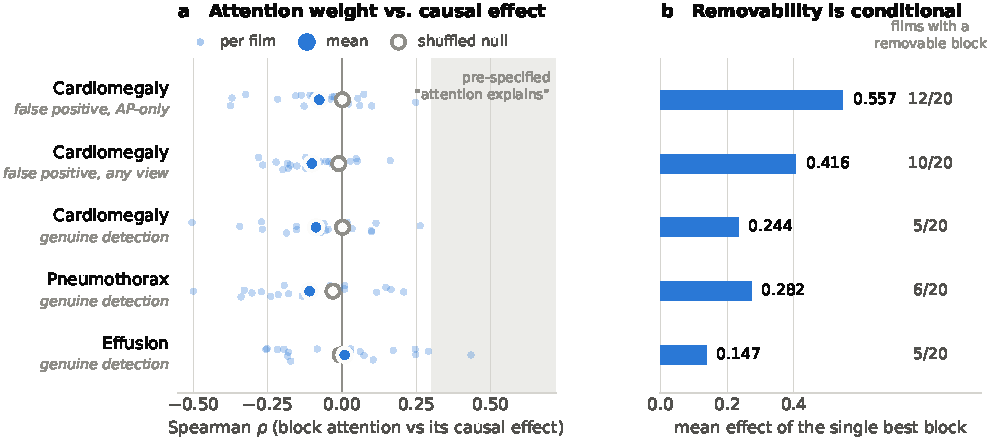
\includegraphics[width=\textwidth]{fig2_generalisation.pdf}
\caption{\textbf{Three findings, two detection regimes.} \textbf{(a)} Within-radiograph Spearman
$\rho$ between a block's attention weight and its causal effect (small dots, one per radiograph;
filled marker, the mean), against a shuffled-attention null (open marker). Every cell is far from
the pre-specified $\rho \ge 0.3$. \textbf{(b)} Mean effect of the single most damaging
block, with the number of radiographs where it moves $\Pnorm$ by more than $0.15$. $20$ radiographs
per cell.}
\label{fig:general}
\end{figure}

Using occlusion maps made the same way, on separate pilot sets (not one per patient), we asked whether the attention the answer position pays to a block
predicts that block's causal effect. It does not, in any of five cells: $\rho$ ranges from \val{attn.rhomin}
to \val{attn.rhomax} against shuffled controls of \val{attn.shufmin} to \val{attn.shufmax}
(Figure~\ref{fig:general}), and four of the five are slightly negative.
\citet{sadanandan2026attention} report the same dissociation in MedGemma at larger scale: on 474
PadChest radiographs their intervals lie below zero, which they read as anticorrelation, and on
VinDr-CXR their correlations are near zero and positive. Our cells have no intervals; a per-patch
analysis on \val{attn.perpatch.n} of the false-positive radiographs gives mean $\rho =
\val{attn.perpatch.ci}$ (film bootstrap, computed after the run) against \val{attn.perpatch.shuf} for
shuffled attention. The interval contains $0$; with \val{attn.perpatch.n} radiographs it cannot
exclude a weak anticorrelation.

Single-block removability depends on the population. It is highest for AP-view false positives
(\val{attn.apfp.best}, \val{attn.apfp.nrem} of \val{attn.apfp.n} radiographs), the population on which an acquisition shortcut would act
\citep{zech2018,degrave2021}; lower across all views (\val{attn.fp.best}, \val{attn.fp.nrem}/\val{attn.fp.n}); and lowest for genuine
detections (\val{attn.tpcard.best}, \val{attn.tpcard.nrem}/\val{attn.tpcard.n}). For effusion and pneumothorax the best block can remove the call
entirely on individual radiographs (\val{attn.eff.bestmax}, \val{attn.ptx.bestmax}) while doing nothing on most.

\begin{center}\small
\begin{tabular}{llccc}
\toprule
Finding & Selection & best block & removable & $\rho$ (shuffled) \\
\midrule
Cardiomegaly & false positive, AP only & \val{attn.apfp.best} & \val{attn.apfp.nrem}/\val{attn.apfp.n} & \val{attn.apfp.rho} \ (\val{attn.apfp.shuf}) \\
Cardiomegaly & false positive, any view & \val{attn.fp.best} & \val{attn.fp.nrem}/\val{attn.fp.n} & \val{attn.fp.rho} \ (\val{attn.fp.shuf}) \\
Cardiomegaly & genuine detection & \val{attn.tpcard.best} & \val{attn.tpcard.nrem}/\val{attn.tpcard.n} & \val{attn.tpcard.rho} \ (\val{attn.tpcard.shuf}) \\
Pneumothorax & genuine detection & \val{attn.tpptx.best} & \val{attn.tpptx.nrem}/\val{attn.tpptx.n} & \val{attn.tpptx.rho} \ (\val{attn.tpptx.shuf}) \\
Effusion & genuine detection & \val{attn.tpeff.best} & \val{attn.tpeff.nrem}/\val{attn.tpeff.n} & \val{attn.tpeff.rho} \ (\val{attn.tpeff.shuf}) \\
\bottomrule
\end{tabular}
\end{center}

\section{Donor sets and amplification}
\label{app:donors}

\begin{table}[h]
\centering
\small
% generated by paper/make_numbers.py; do not edit
\begin{tabular}{lccc}
\toprule
Selection rule & $N{=}20$ & $N{=}80$ & $N{=}320$ \\
\midrule
Top activation & 0.770 & 0.944 & 0.939 \\
Contrast, positive minus negative donors & 0.194 & 0.284 & 0.331 \\
\bottomrule
\end{tabular}

\caption{\textbf{Mean pairwise Jaccard overlap} between the feature sets for cardiomegaly, effusion
and pneumothorax, by selection rule and set size. Patient-disjoint donors, \val{e3.ndonor} per
finding.}
\label{tab:jaccard}
\end{table}

\val{e3.nfilms} cardiomegaly-negative films, selected by $0.05 < \Praw < 0.5$; each $N{=}80$ set
amplified ten times at image positions. Following the pilot study's design, the test scored
first-token readouts only; no answers were sampled. Mean rise in the probability of cardiomegaly:

\begin{center}\small
% generated by paper/make_numbers.py; do not edit
\begin{tabular}{lcc}
\toprule
Feature set & rise in $\Pnorm$ & rise in $\Praw$ \\
\midrule
Cardiomegaly donors & 0.051 & 0.098 \\
Effusion donors & 0.042 & 0.089 \\
Pneumothorax donors & 0.056 & 0.107 \\
The film's own top $80$ & 0.045 & 0.074 \\
Random $80$ & 0.007 & 0.005 \\
\bottomrule
\end{tabular}

\end{center}

Amplifying any set raises the probability a little, and about equally whichever finding's donors it
came from. The pilot study's draw, whose donor sets shared a patient, gave larger rises
(\val{e3.old.card}, \val{e3.old.eff} and \val{e3.old.ptx} in $\Praw$). With patient-disjoint donors
the cardiomegaly set beats the effusion set by \val{e3.amp.cardminuseff} on $\Pnorm$ (Wilcoxon
$p = \val{e3.amp.p.eff}$) and does not beat the pneumothorax set ($p = \val{e3.amp.p.ptx}$).

\section{Evaluation without an intervention}
\label{app:e6}

\begin{table}[h]
\centering
\footnotesize
\setlength{\tabcolsep}{3pt}
% generated by paper/make_numbers.py; do not edit
\begin{tabular}{lcccccc}
\toprule
& \multicolumn{4}{c}{AUC} & \multicolumn{2}{c}{AUC minus AUC of $s$} \\
\cmidrule(lr){2-5}\cmidrule(lr){6-7}
Finding (pos/neg) & $\Praw$ & $\Pnorm$ & $s$ & greedy & $\Praw$ & $\Pnorm$ \\
\midrule
\multicolumn{7}{l}{\emph{MedGemma 1.5 4B}} \\
Cardiomegaly (93/93) & 0.921 & 0.925 & 0.883 & 0.832 & $+0.038$ {\scriptsize$[+0.010,\,+0.067]$} & $+0.042$ {\scriptsize$[+0.016,\,+0.069]$} \\
Effusion (100/100) & 0.857 & 0.851 & 0.809 & 0.799 & $+0.048$ {\scriptsize$[+0.021,\,+0.077]$} & $+0.042$ {\scriptsize$[+0.013,\,+0.071]$} \\
Pneumothorax (57/57) & 0.622 & 0.625 & 0.685 & 0.643 & $-0.064$ {\scriptsize$[-0.126,\,-0.002]$} & $-0.060$ {\scriptsize$[-0.121,\,+0.002]$} \\
\midrule
\multicolumn{7}{l}{\emph{CheXagent-2 3B}} \\
Cardiomegaly (93/93) & 0.955 & 0.955 & 0.954 & 0.866 & $+0.001$ {\scriptsize$[-0.008,\,+0.009]$} & $+0.001$ {\scriptsize$[-0.008,\,+0.008]$} \\
Effusion (100/100) & 0.880 & 0.880 & 0.865 & 0.830 & $+0.016$ {\scriptsize$[+0.003,\,+0.030]$} & $+0.016$ {\scriptsize$[+0.002,\,+0.030]$} \\
Pneumothorax (57/57) & 0.863 & 0.864 & 0.834 & 0.728 & $+0.028$ {\scriptsize$[+0.003,\,+0.056]$} & $+0.030$ {\scriptsize$[+0.005,\,+0.058]$} \\
\bottomrule
\end{tabular}

\caption{\textbf{One evaluation, scored four ways, in two models.} Area under the ROC curve against
the ChestX-ray14 label, for $\Praw$, $\Pnorm$, the sampled yes rate $s$ and the greedy answer (yes
$1$, no $0$, neither $0.5$). Positive and negative radiographs per finding in brackets, one per
patient within each class, the same radiographs for both models. The last two columns, the pre-registered
comparisons, give a readout's AUC minus that of $s$, with a paired $95\%$ film-bootstrap interval.
They compare a continuous score with one that takes only \val{e6.mg.nlevels} values.}
\label{tab:eval}
\end{table}

The first test of whether the readout matters without an intervention scored one closed evaluation
four ways (Table~\ref{tab:eval}): for each finding, up to $100$ patients with the label and as many
without, one radiograph per patient, \val{e6.mg.nsamples} samples per radiograph, in MedGemma and
CheXagent-2. In MedGemma the first-token readouts give a higher AUC than the sampled answers for
cardiomegaly and effusion and a lower one for pneumothorax, and the pre-registered verdict is
\val{e6.mg.verdict}; in CheXagent the differences are smaller (\val{e6.cx.verdict}). Across
the models, the sampled answers separate them on effusion and the readouts do not
(\val{e6.rank.verdict}).

After the run we found that the design compared scores of different resolution. $s$ is a fraction
of \val{e6.mg.nsamples} samples, and MedGemma gives the same answer on all of them for
\val{e6.mg.tiedmin} to \val{e6.mg.tiedmax} of radiographs (CheXagent \val{e6.cx.tiedmin} to
\val{e6.cx.tiedmax}). $s$ ties these radiographs, and a continuous readout still ranks them: among
the \val{e6.mg.card.s0n} cardiomegaly radiographs on which all of MedGemma's samples say no, $\Praw$
alone separates the \val{e6.mg.card.s0pos} positives from the negatives with AUC
\val{e6.mg.card.s0auc}. An analysis chosen after seeing the data, which replaced each readout by
\val{e6.mg.nsamples} simulated answers drawn at its probability, removed the differences (at most
\val{e6.res.maxabs}, every interval containing $0$, in both models). Because that analysis was
chosen after the fact, we tested the question again with matched resolution, on new patients, under
a rule committed before the run.

\begin{table}[h]
\centering
\footnotesize
\setlength{\tabcolsep}{2.5pt}
% generated by paper/make_numbers.py; do not edit
\begin{tabular}{lcccccc}
\toprule
& \multicolumn{3}{c}{AUC} & \multicolumn{3}{c}{AUC of $s$ minus} \\
\cmidrule(lr){2-4}\cmidrule(lr){5-7}
Finding & $\Praw$ & $\Pnorm$ & $s$ & AUC of $\Praw$ & $\mathbb{E}\,$AUC of $q_{\text{raw}}$ & $\mathbb{E}\,$AUC of $q_{\text{norm}}$ \\
\midrule
\multicolumn{7}{l}{\emph{MedGemma 1.5 4B}} \\
Cardiomegaly & 0.886 & 0.885 & 0.854 & $-0.032$ {\scriptsize$[-0.061,\,-0.006]$} & $+0.003$ {\scriptsize$[-0.017,\,+0.025]$} & $-0.007$ {\scriptsize$[-0.031,\,+0.016]$} \\
Effusion & 0.825 & 0.812 & 0.784 & $-0.041$ {\scriptsize$[-0.074,\,-0.011]$} & $+0.013$ {\scriptsize$[-0.016,\,+0.043]$} & $+0.014$ {\scriptsize$[-0.013,\,+0.043]$} \\
Pneumothorax & 0.672 & 0.666 & 0.629 & $-0.043$ {\scriptsize$[-0.105,\,+0.023]$} & $+0.023$ {\scriptsize$[-0.022,\,+0.070]$} & $+0.017$ {\scriptsize$[-0.028,\,+0.061]$} \\
\midrule
\multicolumn{7}{l}{\emph{CheXagent-2 3B}} \\
Cardiomegaly & 0.903 & 0.904 & 0.904 & $+0.000$ {\scriptsize$[-0.010,\,+0.009]$} & $-0.001$ {\scriptsize$[-0.009,\,+0.006]$} & $-0.001$ {\scriptsize$[-0.009,\,+0.006]$} \\
Effusion & 0.850 & 0.850 & 0.847 & $-0.002$ {\scriptsize$[-0.011,\,+0.008]$} & $-0.000$ {\scriptsize$[-0.010,\,+0.010]$} & $-0.000$ {\scriptsize$[-0.010,\,+0.010]$} \\
Pneumothorax & 0.862 & 0.862 & 0.845 & $-0.018$ {\scriptsize$[-0.042,\,+0.007]$} & $-0.005$ {\scriptsize$[-0.028,\,+0.016]$} & $-0.005$ {\scriptsize$[-0.028,\,+0.016]$} \\
\bottomrule
\end{tabular}

\caption{\textbf{One evaluation, scored from the first token and from the written answers, on new
patients.} AUC against the ChestX-ray14 label for $\Praw$, $\Pnorm$ and the sampled yes rate $s$;
\val{e7.nper} positive and \val{e7.nper} negative radiographs per finding, one per patient within
each class (\val{e7.nfilms} radiographs from \val{e7.npat} patients in all), the same radiographs for
both models. The first difference is the comparison of the first evaluation test,
unmatched in resolution. The last two are $D$: the AUC of $s$ minus the expected AUC of $q$, the yes
rate of \val{e7.nsamples} answers drawn at the readout's probability, which is $0$ when the answers
follow the readout. Mean with $95\%$ film-bootstrap interval (\val{e7.nboot} resamples).}
\label{tab:e7}
\end{table}

\paragraph{The matched test.} If the written answers were independent draws at a readout's probability $P$, the yes rate
of $n$ samples would be $q \sim \mathrm{Binomial}(n, P)/n$. We compute the expected AUC of $q$
exactly and test $D = \mathrm{AUC}(s) - \mathbb{E}[\mathrm{AUC}(q)]$, which is $0$ when the answers
follow the readout, under the first test's rule and margin of $0.03$ (Appendix~\ref{app:rules}). The test used \val{e7.npat} patients
not used elsewhere in this paper, \val{e7.nsamples} samples per radiograph and the first test's
generation code unchanged, in MedGemma and in CheXagent-2 3B \citep{chexagent2024}, a
chest-radiograph VLM from a different developer that answers at the first token (answer mass
\val{e7.cx.massmin}, against \val{e7.mg.massmin} to \val{e7.mg.massmax} for MedGemma).
The pre-registered verdict is \val{e7.cx.verdict} in CheXagent and \val{e7.mg.verdict} in
MedGemma (Table~\ref{tab:e7}). Matching resolution shrinks MedGemma's
differences from \val{e7.mg.gapmin}--\val{e7.mg.gapmax} to at most \val{e7.maxabsD}, and every
interval contains $0$, but the intervals reach \val{e7.mg.maxbound}, wider than the margin. They are
wider than planned because, as we found after the run, MedGemma's yes count falls outside the central
$95\%$ of that binomial on \val{e7.mg.outbinmin} to \val{e7.mg.outbinmax} of radiographs (CheXagent
\val{e7.cx.outbinmin} to \val{e7.cx.outbinmax}), which the planning simulation assumed away. Without an intervention, then, we find
no difference in how the readout and the written answers rank radiographs in either model, although
in MedGemma differences up to \val{e7.mg.maxbound} are not excluded. The unmatched comparison again
gives \val{e7.mg.e6rule} in MedGemma, so resolution must be matched. Across the models, reported
without a verdict, $s$ and both matched readouts rank CheXagent-2 above MedGemma on every finding,
each interval excluding $0$ (pneumothorax: \val{e7.rank.ptx.s} under $s$, \val{e7.rank.ptx.qnorm}
under $\Pnorm$); with matched resolution the first test's \val{e6.rank.verdict} does not recur.

\section{Further tables}
\label{app:tables}

\begin{table}[h]
\centering
\footnotesize
\setlength{\tabcolsep}{3pt}
% generated by paper/make_numbers.py; do not edit
\begin{tabular}{lccccc}
\toprule
& & & \multicolumn{3}{c}{drop in $s$} \\
\cmidrule(lr){4-6}
& & & & \multicolumn{2}{c}{correct calls} \\
Feature set & active & in top $80$ & false positives & cardiomegaly & effusion \\
\midrule
Own top $80$ (the paper's) & $80$ & $80$ & $+0.23$ {\scriptsize$[+0.16,\,+0.30]$} & $+0.04$ {\scriptsize$[+0.02,\,+0.07]$} & $+0.17$ {\scriptsize$[+0.06,\,+0.30]$} \\
Cardiomegaly contrast & $80$ & $25$ & $+0.07$ {\scriptsize$[+0.03,\,+0.11]$} & $+0.00$ {\scriptsize$[+0.00,\,+0.01]$} & $+0.03$ {\scriptsize$[+0.01,\,+0.06]$} \\
Effusion contrast & $80$ & $25$ & $+0.04$ {\scriptsize$[+0.02,\,+0.06]$} & $+0.00$ {\scriptsize$[-0.01,\,+0.01]$} & $+0.02$ {\scriptsize$[-0.01,\,+0.06]$} \\
Random active $80$ & $80$ & $4$ & $+0.04$ {\scriptsize$[+0.01,\,+0.07]$} & $-0.00$ {\scriptsize$[-0.01,\,+0.00]$} & $+0.03$ {\scriptsize$[-0.00,\,+0.08]$} \\
Anchored, evidence block & $80$ & $68$ & $+0.27$ {\scriptsize$[+0.19,\,+0.36]$} & $+0.09$ {\scriptsize$[+0.02,\,+0.19]$} & $+0.37$ {\scriptsize$[+0.21,\,+0.53]$} \\
Anchored, border block & $80$ & $68$ & $+0.19$ {\scriptsize$[+0.13,\,+0.26]$} & $+0.02$ {\scriptsize$[+0.01,\,+0.04]$} & $+0.10$ {\scriptsize$[+0.04,\,+0.19]$} \\
\bottomrule
\end{tabular}

\caption{\textbf{Suppressing $80$ features chosen in different ways} (\texttt{scale}~$-1$). Drop in
the sampled yes rate $s$, mean with $95\%$ film-bootstrap interval, from a separate run with
\val{e5.nsamples} samples per film, so the top-$80$ row differs slightly from Table~\ref{tab:v1}. Contrast sets: the $80$ features
whose mean activation differs most between \val{e5.ndonor} positive and \val{e5.ndonor} negative
donor radiographs, one set for all films. Anchored sets: the $80$ most active features over the four
tokens of the film's evidence block, or of a border block. ``Active'' is the mean number of the $80$
active on the film and ``in top $80$'' the mean overlap with the film's own set, both on the false
positives.}
\label{tab:e5}
\end{table}

On correct calls the contrast sets lower $s$ by \val{e5.tpcard.concard.sdrop} (cardiomegaly set,
cardiomegaly calls) and \val{e5.tpeff.coneff.sdrop} (effusion set, effusion calls); on the false
positives $80$ random active features lower it by \val{e5.fp.rand.sdrop}. Anchoring the selection
at the evidence block instead of a border block (sharing \val{e5.fp.evid.overlap} features with the
top set) leans toward larger drops: \val{e5.S3.ci} on the false positives (\val{e5.S3}, short of the
pre-registered $0.10$) and \val{e5.S3.tpeff.ci} on correct effusion calls (no verdict).

\paragraph{Prompt phrasings.} A pilot-study test, kept for the record (Appendix~\ref{app:rules}):
four phrasings of the cardiomegaly question on \val{ps.n} radiographs, first-token readouts only.
Its rule asked whether a phrasing shifts $\Praw$ by more than $0.15$ while shifting $\Pnorm$ by less
than $0.05$, and none does. The rule did not test direction: dropping the format instruction lowers
the answer mass from \val{ps.plain.mass} to \val{ps.noformat.mass} and moves the two readouts in
opposite directions ($\Praw$ \val{ps.noformat.draw}, $\Pnorm$ \val{ps.noformat.dnorm}). No written
answers were scored in this test, so which readout follows them is unknown.

\begin{center}
\small
\begin{tabular}{lccccc}
\toprule
Phrasing & $\Praw$ & $\Pnorm$ & $m$ & change in $\Praw$ & change in $\Pnorm$ \\
\midrule
Plain & \val{ps.plain.raw} & \val{ps.plain.norm} & \val{ps.plain.mass} & -- & -- \\
No format instruction & \val{ps.noformat.raw} & \val{ps.noformat.norm} & \val{ps.noformat.mass} & \val{ps.noformat.draw} & \val{ps.noformat.dnorm} \\
Radiologist persona & \val{ps.persona.raw} & \val{ps.persona.norm} & \val{ps.persona.mass} & \val{ps.persona.draw} & \val{ps.persona.dnorm} \\
Finding defined & \val{ps.gloss.raw} & \val{ps.gloss.norm} & \val{ps.gloss.mass} & \val{ps.gloss.draw} & \val{ps.gloss.dnorm} \\
\bottomrule
\end{tabular}
\end{center}

\paragraph{Compute.} All experiments ran on one H100 (80\,GB). Wall-clock time of each generation
run, from its log in the repository: first check \val{compute.e2} min, replication
\val{compute.e4} min, contrastive selection \val{compute.e5} min, first evaluation
\val{compute.e6mg} min (MedGemma) and \val{compute.e6cx} min (CheXagent), matched evaluation
\val{compute.e7mg} and \val{compute.e7cx} min. Some runs shared the GPU.

\end{document}
